%%%%%%%%%%%%%%%%%%%%%%%%%%%%%%%%%%%%%%%%
% datoteka diploma-FRI-vzorec.tex
%
%POZOR: ta verzija ne producira pdf datoteke v pdf/A formatu!!!
%namenjena je le za nalogo pri Diplomskem seminarju!
%
% vzorčna datoteka za pisanje diplomskega dela v formatu LaTeX
% na UL Fakulteti za računalništvo in informatiko
%
% na osnovi starejših verzij vkup spravil Franc Solina, maj 2021
% prvo verzijo je leta 2010 pripravil Gašper Fijavž
%
% za upravljanje z literaturo ta vezija uporablja BibLaTeX
%
% svetujemo uporabo Overleaf.com - na tej spletni implementaciji LaTeXa ta vzorec pravilno deluje
%

\documentclass[a4paper, 12pt, openright]{book}
%\documentclass[a4paper, 12pt, openright, draft]{book}  %Nalogo preverite tudi z opcijo draft, ki pokaže, katere vrstice so predolge! Pozor, v draft opciji, se slike ne pokažejo!
 
\usepackage[utf8]{inputenc}   % omogoča uporabo slovenskih črk kodiranih v formatu UTF-8
\usepackage[slovene,english]{babel}    % naloži, med drugim, slovenske delilne vzorce
\usepackage{graphicx}  % omogoča vlaganje slik različnih formatov
\graphicspath{{./slike/}}
\usepackage{subcaption}
\usepackage{caption}
\captionsetup{justification=raggedright,singlelinecheck=false}
\usepackage{fancyhdr}          % poskrbi, na primer, za glave strani
\usepackage{amssymb}           % dodatni matematični simboli
\usepackage{amsmath}           % eqref, npr.
\usepackage{hyperxmp}
\usepackage[hyphens]{url}
\usepackage{csquotes}
\usepackage[pdftex, colorlinks=true,
						citecolor=black, filecolor=black, 
						linkcolor=black, urlcolor=black,
						pdfproducer={LaTeX}, pdfcreator={LaTeX}]{hyperref}

\usepackage{color}
\usepackage{soul}

\usepackage{subcaption}

\usepackage[
backend=biber,
style=numeric,
sorting=nty,
]{biblatex}


\addbibresource{literatura.bib} %Imports bibliography file

\usepackage[a-1b]{pdfx}
\usepackage{hyperref}

%%%%%%%%%%%%%%%%%%%%%%%%%%%%%%%%%%%%%%%%
%	CUSTOM COMMANDS
%%%%%%%%%%%%%%%%%%%%%%%%%%%%%%%%%%%%%%%%
\newcommand{\en}{angl.}
\newcommand{\comment}[1]{}

%%%%%%%%%%%%%%%%%%%%%%%%%%%%%%%%%%%%%%%%
%	DIPLOMA INFO
%%%%%%%%%%%%%%%%%%%%%%%%%%%%%%%%%%%%%%%%
\newcommand{\ttitle}{Avtomatska transkripcija klavirske glasbe s konvolucijskimi nevronskimi mrežami}
\newcommand{\ttitleEn}{Automatic music transcription of piano music with convolutional neural networks}
\newcommand{\tsubject}{\ttitle}
\newcommand{\tsubjectEn}{\ttitleEn}
\newcommand{\tauthor}{Domen Mohorčič}

\newcommand{\tmentor}{prof. dr. Igor Kononenko}
\newcommand{\tcomentor}{doc. dr. Matevž Pesek}

\newcommand{\tkeywords}{avtomatska transkripcija glasbe, konvolucijska nevronska mreža, klavirska glasba, transformacija s konstantnim Q, logaritemska kompresija}
\newcommand{\tkeywordsEn}{automatic music transcription, convolutional neural network, piano music, constant Q transform, logarithmic compression}

%%%%%%%%%%%%%%%%%%%%%%%%%%%%%%%%%%%%%%%%
%	HYPERREF SETUP
%%%%%%%%%%%%%%%%%%%%%%%%%%%%%%%%%%%%%%%%
\hypersetup{pdftitle={\ttitle}}
\hypersetup{pdfsubject=\ttitleEn}
\hypersetup{pdfauthor={\tauthor, dm4492@fri.uni-lj.si}}
\hypersetup{pdfkeywords=\tkeywordsEn}

%%%%%%%%%%%%%%%%%%%%%%%%%%%%%%%%%%%%%%%%
% postavitev strani
%%%%%%%%%%%%%%%%%%%%%%%%%%%%%%%%%%%%%%%%  

\addtolength{\marginparwidth}{-20pt} % robovi za tisk
\addtolength{\oddsidemargin}{40pt}
\addtolength{\evensidemargin}{-40pt}

\renewcommand{\baselinestretch}{1.3} % ustrezen razmik med vrsticami
\setlength{\headheight}{15pt}        % potreben prostor na vrhu
\renewcommand{\chaptermark}[1]%
{\markboth{\MakeUppercase{\thechapter.\ #1}}{}} \renewcommand{\sectionmark}[1]%
{\markright{\MakeUppercase{\thesection.\ #1}}} \renewcommand{\headrulewidth}{0.5pt} \renewcommand{\footrulewidth}{0pt}
\fancyhf{}
\fancyhead[LE,RO]{\sl \thepage} 
%\fancyhead[LO]{\sl \rightmark} \fancyhead[RE]{\sl \leftmark}
\fancyhead[RE]{\sc \tauthor}              % dodal Solina
\fancyhead[LO]{\sc Diplomska naloga}     % dodal Solina


\newcommand{\BibLaTeX}{{\sc Bib}\LaTeX}
\newcommand{\BibTeX}{{\sc Bib}\TeX}

%%%%%%%%%%%%%%%%%%%%%%%%%%%%%%%%%%%%%%%%
% naslovi
%%%%%%%%%%%%%%%%%%%%%%%%%%%%%%%%%%%%%%%%  

\newcommand{\autfont}{\Large}
\newcommand{\titfont}{\LARGE\bf}
\newcommand{\clearemptydoublepage}{\newpage{\pagestyle{empty}\cleardoublepage}}
\setcounter{tocdepth}{1}	      % globina kazala

%%%%%%%%%%%%%%%%%%%%%%%%%%%%%%%%%%%%%%%%
% konstrukti
%%%%%%%%%%%%%%%%%%%%%%%%%%%%%%%%%%%%%%%%  
\newtheorem{izrek}{Izrek}[chapter]
\newtheorem{trditev}{Trditev}[izrek]
\newenvironment{dokaz}{\emph{Dokaz.}\ }{\hspace{\fill}{$\Box$}}


%%%%%%%%%%%%%%%%%%%%%%%%%%%%%%%%%%%%%%%%%%%%%%%%%%%%%%%%%%%%%%%%%%%%%%%%%%%%%%%
%% PDF-A
%%%%%%%%%%%%%%%%%%%%%%%%%%%%%%%%%%%%%%%%%%%%%%%%%%%%%%%%%%%%%%%%%%%%%%%%%%%%%%%

%%%%%%%%%%%%%%%%%%%%%%%%%%%%%%%%%%%%%%%% 
% define medatata
%%%%%%%%%%%%%%%%%%%%%%%%%%%%%%%%%%%%%%%% 
%\def\Title{\ttitle}
%\def\Author{\tauthor, matjaz.kralj@fri.uni-lj.si}
%\def\Subject{\ttitleEn}
%\def\Keywords{\tkeywordsEn}

%%%%%%%%%%%%%%%%%%%%%%%%%%%%%%%%%%%%%%%% 
% \convertDate converts D:20080419103507+02'00' to 2008-04-19T10:35:07+02:00
%%%%%%%%%%%%%%%%%%%%%%%%%%%%%%%%%%%%%%%% 

%%%%%%%%%%%%%%%%%%%%%%%%%%%%%%%%%%%%%%%%
% get pdftex version string
%%%%%%%%%%%%%%%%%%%%%%%%%%%%%%%%%%%%%%%% 
\newcount\countA
\countA=\pdftexversion
\advance \countA by -100
\def\pdftexVersionStr{pdfTeX-1.\the\countA.\pdftexrevision}


%%%%%%%%%%%%%%%%%%%%%%%%%%%%%%%%%%%%%%%%
% XMP data
%%%%%%%%%%%%%%%%%%%%%%%%%%%%%%%%%%%%%%%%  
%\usepackage{xmpincl}
%\includexmp{pdfa-1b}

%%%%%%%%%%%%%%%%%%%%%%%%%%%%%%%%%%%%%%%%
% pdfInfo
%%%%%%%%%%%%%%%%%%%%%%%%%%%%%%%%%%%%%%%%  
\pdfinfo{%
    /Title    (\ttitle)
    /Author   (\tauthor, dm4492@student.uni-lj.si)
    /Subject  (\ttitleEn)
    /Keywords (\tkeywordsEn)
    /ModDate  (\pdfcreationdate)
    /Trapped  /False
}

%%%%%%%%%%%%%%%%%%%%%%%%%%%%%%%%%%%%%%%%
% znaki za copyright stran
%%%%%%%%%%%%%%%%%%%%%%%%%%%%%%%%%%%%%%%%  

\newcommand{\CcImageCc}[1]{%
	
\includegraphics[scale=#1]{cc_cc_30.pdf}%
}
\newcommand{\CcImageBy}[1]{%
	
\includegraphics[scale=#1]{cc_by_30.pdf}%
}
\newcommand{\CcImageSa}[1]{%
	
\includegraphics[scale=#1]{cc_sa_30.pdf}%
}

%%%%%%%%%%%%%%%%%%%%%%%%%%%%%%%%%%%%%%%%%%%%%%%%%%%%%%%%%%%%%%%%%%%%%%%%%%%%%%%
%%%%%%%%%%%%%%%%%%%%%%%%%%%%%%%%%%%%%%%%%%%%%%%%%%%%%%%%%%%%%%%%%%%%%%%%%%%%%%%

\begin{document}
\selectlanguage{slovene}
\frontmatter
\setcounter{page}{1} %
\renewcommand{\thepage}{}       % preprečimo težave s številkami strani v kazalu

%%%%%%%%%%%%%%%%%%%%%%%%%%%%%%%%%%%%%%%%
%naslovnica
 \thispagestyle{empty}%
   \begin{center}
    {\large\sc Univerza v Ljubljani\\%
%      Fakulteta za elektrotehniko\\% za študijski program Multimedija
%      Fakulteta za upravo\\% za študijski program Upravna informatika
      Fakulteta za računalništvo in informatiko\\%
%      Fakulteta za matematiko in fiziko\\% za študijski program Računalništvo in matematika
     }
    \vskip 10em%
    {\autfont \tauthor \par}%
    {\titfont \ttitle \par}%
    {\vskip 3em \textsc{DIPLOMSKO DELO\\[5mm]         % dodal Solina za ostale študijske programe
%    VISOKOŠOLSKI STROKOVNI ŠTUDIJSKI PROGRAM\\ PRVE STOPNJE\\ RAČUNALNIŠTVO IN INFORMATIKA}\par}%
     UNIVERZITETNI  ŠTUDIJSKI PROGRAM\\ PRVE STOPNJE\\ RAČUNALNIŠTVO IN INFORMATIKA}\par}%
%    INTERDISCIPLINARNI UNIVERZITETNI\\ ŠTUDIJSKI PROGRAM PRVE STOPNJE\\ MULTIMEDIJA}\par}%
%    INTERDISCIPLINARNI UNIVERZITETNI\\ ŠTUDIJSKI PROGRAM PRVE STOPNJE\\ UPRAVNA INFORMATIKA}\par}%
%    INTERDISCIPLINARNI UNIVERZITETNI\\ ŠTUDIJSKI PROGRAM PRVE STOPNJE\\ RAČUNALNIŠTVO IN MATEMATIKA}\par}%
    \vfill\null%
% izberite pravi habilitacijski naziv mentorja!
    {\large \textsc{Mentor}: \tmentor \par}%
    {\large \textsc{Somentor}: \tcomentor \par}%
    {\vskip 2em \large Ljubljana, \the\year \par}%
\end{center}
% prazna stran
%\clearemptydoublepage      
% izjava o licencah itd. se izpiše na hrbtni strani naslovnice

%%%%%%%%%%%%%%%%%%%%%%%%%%%%%%%%%%%%%%%%
%copyright stran
%%%%%%%%%%%%%%%%%%%%%%%%%%%%%%%%%%%%%%%%
\newpage
\thispagestyle{empty}

\vspace*{5cm}
{\small \noindent
To delo je ponujeno pod licenco \textit{Creative Commons Priznanje avtorstva-Deljenje pod enakimi pogoji 2.5 Slovenija} (ali novej\v so razli\v cico).
To pomeni, da se tako besedilo, slike, grafi in druge sestavine dela kot tudi rezultati diplomskega dela lahko prosto distribuirajo,
reproducirajo, uporabljajo, priobčujejo javnosti in predelujejo, pod pogojem, da se jasno in vidno navede avtorja in naslov tega
dela in da se v primeru spremembe, preoblikovanja ali uporabe tega dela v svojem delu, lahko distribuira predelava le pod
licenco, ki je enaka tej.
Podrobnosti licence so dostopne na spletni strani \href{http://creativecommons.si}{creativecommons.si} ali na Inštitutu za
intelektualno lastnino, Streliška 1, 1000 Ljubljana.

\begin{center}% 0.66 / 0.89 = 0.741573033707865
\CcImageCc{0.741573033707865}\hspace*{1ex}\CcImageBy{1}\hspace*{1ex}\CcImageSa{1}%
\end{center}
}

\vspace*{1.5cm}
{\small \noindent
Izvorna koda diplomskega dela, njeni rezultati in v ta namen razvita programska oprema je ponujena pod licenco GNU General Public License,
različica 3 (ali novejša). To pomeni, da se lahko prosto distribuira in/ali predeluje pod njenimi pogoji.
Podrobnosti licence so dostopne na spletni strani \url{http://www.gnu.org/licenses/}.
}

\vfill
\begin{center} 
\ \\ \vfill
{\em
Besedilo je oblikovano z urejevalnikom besedil \LaTeX.}
\end{center}

% prazna stran
\clearemptydoublepage

%%%%%%%%%%%%%%%%%%%%%%%%%%%%%%%%%%%%%%%%
% stran 3 med uvodnimi listi
\thispagestyle{empty}
\
\vfill

\bigskip
\noindent\textbf{Kandidat:} \tauthor \\
\noindent\textbf{Naslov:} \ttitle \\
% vstavite ustrezen naziv študijskega programa!
\noindent\textbf{Vrsta naloge:} Diplomska naloga na univerzitetnem programu prve stopnje Računalništvo in informatika \\
% izberite pravi habilitacijski naziv mentorja!
\noindent\textbf{Mentor:} \tmentor \\
\noindent\textbf{Somentor:} \tcomentor

\bigskip
\noindent\textbf{Opis:}\\
Avtomatska transkripcija glasbe je algoritmičnen zapis not iz glasbenega posnetka.
Kandidat naj analizira trenutno stanje na področju avtomatske transkripcije glasbe s pomočjo strojnega učenja, kjer naj se osredotoči predvsem na konvolucijske nevronske mreže.
Preizkusi in primerja naj več različnih arhitektur in velikosti konvolucijskih nevronskih mrež na zbirki posnetkov klavirske glasbe.
Pri tem naj poskuša ugotoviti, katera vrsta normalizacije spektrogramov je bolj ustrezna za tovrstno transkripcijo.

%\bigskip
%\noindent\textbf{Title:} Automatic music transcription of piano music with convolution neural networks

%\bigskip
%\noindent\textbf{Description:}\\
%opis diplome v angleščini

\vfill



\vspace{2cm}

% prazna stran
\clearemptydoublepage

% zahvala
\thispagestyle{empty}\mbox{}\vfill\null\it%
\noindent
%Na tem mestu zapišite, komu se zahvaljujete za izdelavo diplomske naloge. Pazite, da ne boste koga pozabili. Utegnil vam bo zameriti. Temu se da izogniti tako, da celotno zahvalo izpustite.
Zahvaljujem se svojima mentorjema za vse nasvete in pomoč pri izdelavi te diplomske naloge.
Zahvaljujem se tudi svoji punci Niki in družini, ki so mi stali ob strani, razumeli mojo zaposlenost z diplomsko nalogo in me podpirali pri študiju.
\rm\normalfont

% prazna stran
\clearemptydoublepage

%%%%%%%%%%%%%%%%%%%%%%%%%%%%%%%%%%%%%%%%
% posvetilo, če sama zahvala ne zadošča :-)
%\thispagestyle{empty}\mbox{}{\vskip0.20\textheight}\mbox{}\hfill\begin{minipage}{0.55\textwidth}%
%Posvetilo
%\normalfont\end{minipage}

% prazna stran
%\clearemptydoublepage


%%%%%%%%%%%%%%%%%%%%%%%%%%%%%%%%%%%%%%%%
% kazalo
\pagestyle{empty}
\def\thepage{}% preprečimo težave s številkami strani v kazalu
\tableofcontents{}


% prazna stran
%\clearemptydoublepage


%%%%%%%%%%%%%%%%%%%%%%%%%%%%%%%%%%%%%%%%
% seznam kratic

\chapter*{Seznam uporabljenih kratic}

\noindent\begin{tabular}{p{0.11\textwidth}|p{.39\textwidth}|p{.39\textwidth}} % po potrebi razširi prvo kolono tabele na račun drugih dveh!
  {\bf kratica} & {\bf angleško} & {\bf slovensko} \\
  \hline
  \textbf{AMT} & automatic music transcription & avtomatska transkripcija glasbe \\
  \textbf{MIR} & music information retrieval & pridobivanje informacij iz glasbe \\
  \textbf{MPE} & multi-pitch estimation & ocenjevanje tonskih višin \\
  \textbf{NMF} & non-negative matrix factorization & nenegativna matrična faktorizacija \\
  \textbf{HMM} & hidden Markov models & prikriti markovski modeli \\
  \textbf{NN} & neural network & nevronska mreža \\
  \textbf{DNN} & deep neural network & globoka nevronska mreža \\
  \textbf{RNN} & recurrent neural network & nevronska mreža s povratno zanko \\
  \textbf{LSTM} & long short-term memory & dolgi kratkoročni spomin \\
  \textbf{CNN} & convolutional neural network & konvolucijska nevronska mre\-ža \\
  \textbf{DFT} & discreet Fourier transform & diskretna Fourierova transformacija \\
  \textbf{CQT} & constant Q transformation & transformacija s konstantnim Q \\
  \textbf{FFT} & fast Fourier transform & hitra Fourierova transformacija \\
  \textbf{STFT} & short-time Fourier transform & kratko-časovna Fourierova transformacija \\
  \textbf{ReLU} & rectified linear unit & popravljena linearna enota \\
\end{tabular}


% prazna stran
\clearemptydoublepage


%%%%%%%%%%%%%%%%%%%%%%%%%%%%%%%%%%%%%%%%
% povzetek
\addcontentsline{toc}{chapter}{Povzetek}
\chapter*{Povzetek}

\noindent\textbf{Naslov:} \ttitle
\bigskip

\noindent\textbf{Avtor:} \tauthor
\bigskip

%\noindent\textbf{Povzetek:}
%\noindent V vzorcu je predstavljen postopek priprave diplomskega dela z uporabo okolja \LaTeX. Vaš povzetek mora sicer vsebovati približno 100 besed, ta tukaj je odločno prekratek. Dober povzetek vključuje: (1) kratek opis obravnavanega problema, (2) kratek opis vašega pristopa za reševanje tega problema in (3) (najbolj uspešen) rezultat ali prispevek diplomske naloge.
\noindent V diplomski nalogi obravnavamo problem avtomatske transkripcije glasbe z uporabo globokih nevronskih mrež, natančneje s konvolucijskimi nevronskimi mrežami.
Avtomatska transkripcija glasbe je postopek zapisa not iz poslušanja glasbenega posnetka.
Preučili smo dosedanje pristope in ugotovili pomanjkanje raziskav o velikosti in o obliki posameznih arhitektur globokih modelov.
Raziskali smo uspešnost štirih različnih arhitektur konvolucijskih nevronskih mrež na zbirki klavirskih posnetkov MAPS, ki je pogosta izbira za učenje avtomatske transkripcije glasbe.
Preučili smo tudi dva različna pristopa normalizacije spektrogramov: standardizacijo in logaritemsko kompresijo.
Izkazalo se je, da na uspešnost transkripcije pozitivno vpliva večje število konvolucijskih plasti v nevronski mreži.
Prav tako je bila transkripcija na logaritemsko kompresiranih spektrogramih za 10 \% uspešnejša od transkripcije na standardiziranih spektrogramih.

\bigskip

\noindent\textbf{Ključne besede:} \tkeywords.


% prazna stran
\clearemptydoublepage


%%%%%%%%%%%%%%%%%%%%%%%%%%%%%%%%%%%%%%%%
% abstract
\selectlanguage{english}
\addcontentsline{toc}{chapter}{Abstract}
\chapter*{Abstract}

\noindent\textbf{Title:} \ttitleEn
\bigskip

\noindent\textbf{Author:} \tauthor
\bigskip

%\noindent\textbf{Abstract:} 
\noindent In this thesis we explore the problem of automatic music transcription using deep neural networks, more specific convolutional neural networks.
Automatic music transcription is a task of writing the sheet music from musical recordings.
We analysed previous studies and found that there was a lack of research about the size and the shape of architecture of deep models.
We explored the performance of four different architectures of convolutional neural networks on the piano recordings dataset MAPS, which is a common benchmark for learning automatic music transcription.
We also compared two different normalization techniques for spectrograms: standardization and the logarithmic compression.
We found out that the performance of transcription is highly correlated with the higher number of convolutional layers.
Transcription is also 10\% more successful with logarithmic compression instead of standardization.

\bigskip

\noindent\textbf{Keywords:} \tkeywordsEn.
\selectlanguage{slovene}


% prazna stran
\clearemptydoublepage


%%%%%%%%%%%%%%%%%%%%%%%%%%%%%%%%%%%%%%%%
\mainmatter
\setcounter{page}{1}
\pagestyle{fancy}


\chapter{Uvod}

Transkripcija glasbe je postopek, pri katerem se zapiše notni zapis poslušane glasbe.
Kljub temu, da gre za relativno enostaven postopek zapisovanja slišanega, imamo ljudje težave pri zapisovanju poslušanih not, pri čimer so profesionalni glasbeniki med najbolj uspešnimi.
Postopek transkripcije običajno vključuje osebo, ki večkrat posluša isti posnetek in pri tem poskuša zapisati, katere note sliši.
Pri tem pogosto uporabi svoje teoretično glasbeno znanje o kvantiziranih dolžinah not in o tonaliteti glasbe.
Naloga postane zahtevnejša, ko se med glasbo spreminjata hitrost ali tonaliteta, mnogo težja pa postane, ko je v posnetku prisotnih več inštrumentov.
Takrat se oseba najprej posveti enemu inštrumentu, nato drugemu in tako naprej.
Postopek je zelo zamuden, poleg tega pa popolna transkripcija ni vedno mogoča.
Pogosto v določenih delih glasbe nekateri inštrumenti preglasijo druge ali se podvajajo in jih je zato težje ali celo nemogoče slišati.
Zaradi vseh nevšečnosti se je pojavila ideja o avtomatski transkripciji glasbe, kjer bi namesto človeka delo opravljal računalnik.

Avtomatska transkripcija glasbe (\en\ Automatic Music Transcription -- AMT) je postopek, pri katerem računalnik zapiše notni zapis poslušane glasbe.
AMT je eden izmed pomembnejših problemov pri pridobivanju informacij iz glasbe (\en\ Music Information Retrieval -- MIR) \cite{mirex}.
Pri AMT se glasbo pogosto najprej pretvori v spektrogram, ki je vizualna predstavitev amplitud frekvenc v času, na katerem se nato uči izbrani model.
Pri enoglasni glasbi je transkripcija v primerjavi z večglasno glasbo enostavna.
Lahko se uporabi avtokorelacija signala, iz katere se izlušči frekvenca prisotnega tona, imenovana tudi fundamentalna frekvenca.
Pri večglasni glasbi pa je problem mnogo težji.
Frekvence tonov, ki so hkrati prisotne v signalu, povzročijo kompleksne medsebojne interakcije in prekrivanje višjih harmonikov fundamentalnih frekvenc.
Višje harmonske frekvence so načeloma tišje od fundamentalnih frekvenc, vendar tudi to ne drži za vse inštrumente, zato fundamentalnih frekvenc ne moremo določiti z iskanjem najglasnejših frekvenc.
Drugi velik problem je variabilnost vhodnega signala glede na tip inštrumenta.
Različni inštrumenti različno zvenijo in imajo drugačno barvo tona (\en\ timbre), zato se signali in spektrogrami istih skladb, igranih z različnimi inštrumenti, razlikujejo med sabo.
AMT pristopi zaradi tega pogosto uporabljajo kompleksne globoke modele, ki so sposobni razlikovati med frekvencami tonov, harmoniki in potencialno različnimi inštrumenti.

Zaradi vseh težav pri transkripciji glasbe popoln model za večglasno transkripcijo glasbe po vsej verjetnosti ne bo nikoli obstajal, lahko pa naredimo zelo dobre AMT modele za posamezne inštrumente.
Pri tem lahko dober AMT model z visoko točnostjo zaznavanja not nadomesti glasbenega eksperta, s čimer se prihrani ogromno časa pri transkripciji.
Poleg tega se lahko dober AMT model uporabi za digitalizacijo obstoječe posnete glasbe in kasnejše urejanje le-te ali za zapis not improviziranega glasbenega nastopa solista.
Dober AMT model lahko tako v zelo kratkem času transkribira in digitalizira ogromne glasbene zbirke, za kar bi glasbeni eksperti lahko porabili več let.
AMT modele se lahko uporabi tudi za pomoč pri transkripciji, saj nam lahko kot osnovo nudi, kateri toni so prisotni ob določenem času v posnetku.
Glasbeni ekspert si lahko s tem ogromno pomaga, saj potrebuje razbrati samo, kateri toni so pravilni in kateri lažni ter ali kje kaj manjka, zraven pa uporablja svoje glasbeno znanje.
Velikokrat pa so AMT modeli zelo veliki, kompleksni in nepraktični za učenje s časovnega vidika, sploh če nimamo dostopa do boljših računalniških sistemov z veliko zmogljivostjo.
Kljub temu da so kompleksnejši modeli po navadi boljši od enostavnejših, slednji niso veliko slabši od njih.
Raziskav o manjših AMT modelih nismo zasledili, zato o velikosti ne vemo prav dosti. Večina raziskav naredi en model, nič pa ne poročajo o rezultatih pri različnih velikostih modelov.
Zato smo se odločili narediti primerjavo različno velikih AMT modelov.
Najbolj uspešne metode danes vključujejo konvolucijske nevronske mreže, zato smo raziskali, kako velikost konvolucijskih nevronskih mrež vpliva na uspešnost transkripcije.

V diplomskem delu se zato posvečamo avtomatski transkripciji večglasne glasbe s konvolucijskimi nevronskimi mrežami in raziščemo odvisnost med velikostjo modelov in njihovimi rezultati.
Preverili smo, kako priprava podatkov vpliva na uspešnost učenja modelov in ali večji modeli dosegajo bistveno boljše rezultate.
Preverili smo tudi, kako velikost modela vpliva na čas učenja in ali več časa učeni modeli dosegajo boljše rezultate.
V poglavju \ref{ch:background} smo naredili pregled dosedanjih poskusov avtomatske transkripcije glasbe in predstavili najbolj uspešne pristope.
V poglavju \ref{ch:methods} smo predstavili uporabljene metode.
V poglavju \ref{ch:work} smo se osredotočili na podatke in implementacijo.
V poglavju \ref{ch:results} smo pregledali dobljene rezultate in v poglavju \ref{ch:discussion} smo rezultate podrobneje analizirali, naredili zaključke in predlagali nadaljnje izboljšave.


\chapter{Ozadje}
\label{ch:background}

\section{Avtomatska transkripcija glasbe}

Raziskave o avtomatski transkripciji glasbe so se začele v 70-ih letih prejšnjega stoletja in se delijo na štiri kategorije, kot so jih razvrstili Benetos in ostali leta 2019 v \cite{benetos2019overview}: okvirne (\en\ frame-level), notne (\en\ note-level), inštrumentne (\en\ stream-level) in zapisne (\en\ notation-level).
Okvirna transkripcija (\en\ Multi-Pitch Estimation -- MPE) se ukvarja z ugotavljanjem prisotnosti posameznih frekvenc v do\-lo\-če\-nem kratkem časovnem intervalu v posnetku, imenovanem okno. Primer okvirne transkripcije je na sliki \ref{fig:window}.
Metode MPE ne poznajo koncepta not in ne morejo ugotoviti kompleksnejših glasbenih lastnosti, kot sta tempo ali tonaliteta.
Notna transkripcija (sledenje not, \en\ Note Tracking) je nivo višje kot okvirno sledenje.
Notna transkripcija nadgradi okvirno transkripcijo tako, da poveže prisotne frekvence skozi čas v note.
Note so definirane z začetkom (\en\ Onset, start), koncem (\en\ Offset, end), višino tona (\en\ Pitch), in glasnostjo (\en\ Velocity).
Naslednja stopnja nad notno transkripcijo je inštrumentna transkripcija.
Inštrumentna transkripcija združuje note v skupine, kjer vsaka skupina predstavlja posamezen inštrument.
Pri tem si metode pomagajo z dejstvom, da imajo različni inštrumenti različno barvo tona in zato zvenijo različno.
Zapisna transkripcija pa poskuša spremeniti posneto glasbo v zapis, ki je lahko berljiv človeku, na primer notni zapis.
Taki pristopi potrebujejo kompleksno znanje o glasbenih strukturah, kot so tempo, tonaliteta, ritem in akordi.
V tej diplomski nalogi smo se posvetili okvirnim pristopom.

\begin{figure}
    \centering
    \begin{subfigure}[t]{.45\textwidth}
        \centering
        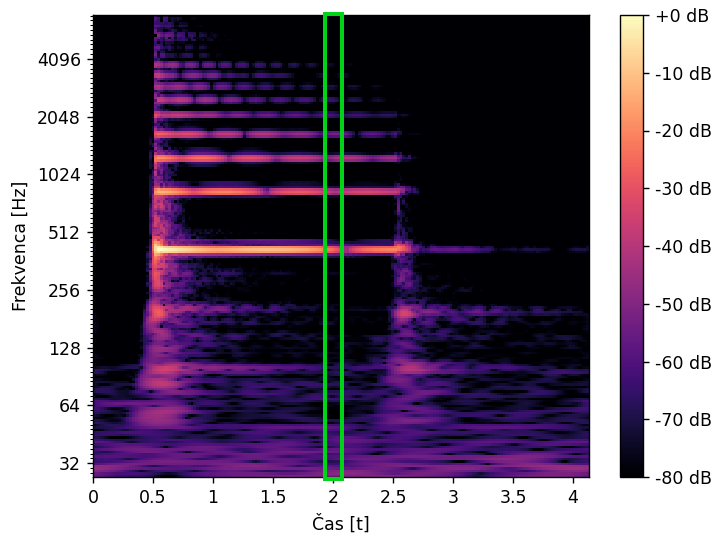
\includegraphics[width=\linewidth]{input.png}
        \caption{CQT spektrogram tona A1 s frekvenco 440 Hz. Na sliki so prisotni tudi višji harmoniki, vendar so časovno in amplitudno šibkejši od fundamentalne frekvence.}
        \label{fig:spec}
    \end{subfigure}%
    \hspace{1em}%
    \begin{subfigure}[t]{.45\textwidth}
        \centering
        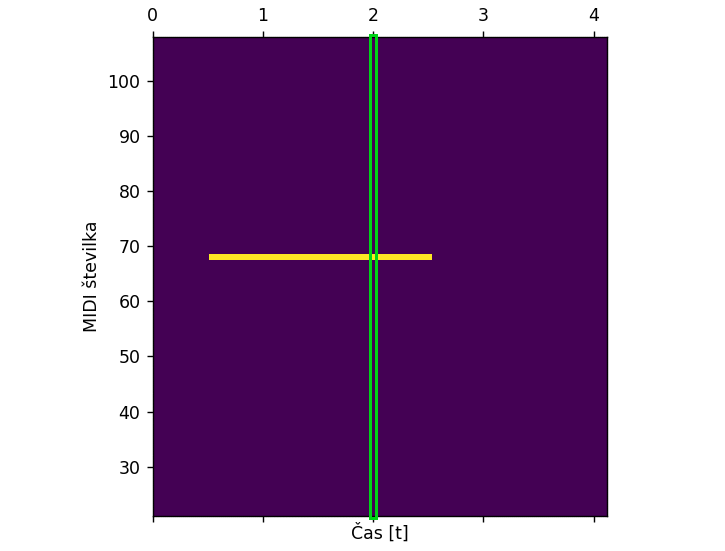
\includegraphics[width=\linewidth]{input_out.png}
        \caption{Označena prisotnost tonskih višin po času. Ton A1, ki ima MIDI številko 69 in se po MIDI nomenklaturi imenuje tudi A4, je na spektrogramu označen z začetkom okoli 0.5 s in koncem okoli 2.5 s.}
        \label{fig:spec_out}
    \end{subfigure}
    \caption{Pri okvirni transkripciji model kot vhod dobi del spektrograma ali okno, ki je označeno z zelenim okvirjem na levi sliki. Izhod modela je vektor, označen z zelenim okvirjem na desni sliki, ki prikazuje, katere klavirske tipke so bile pritisnjene v oknu. Model z oknom drsi po spektrogramu in za vsako postavitev okna vrne vektor prisotnih tonskih višin.}
    \label{fig:window}
\end{figure}

\section{Predhodniki globokega učenja}

Prvi okvirni pristopi so vključevali analizo signalov.
Enega prvih pristopov je opisal Moorer leta 1975 v svojem doktorskem delu \cite{moorer1975digital}.
V njem je opisal pristop za transkripcijo duetov.
Njegov pristop je vključeval frekvenčni detektor in detekor energije signala.
Kjer sta se izhoda detektorjev strinjala, da gre za noto, jo je model zapisal.
Njegov pristop pa je imel nekaj ključnih omejitev.
V duetu sta morala biti dva različna inštrumenta in igrati sta morala na različnih višinah, da ju je metoda lahko ločila med sabo.

Leta 1989 sta na Osaški univerzi v Tokiju, Japonska, raziskovalca Katayose in Inokuchi kot del raziskave počutja v glasbi naredila model zaznavanja fundamentalnih frekvenc večglasne glasbe \cite{katayose1989kensei}.
Njun pristop je iz prvih nekaj sekund posnetka razbral dolžino dobe.
Nato sta izračunala časovno-frekvenčno sliko in samo ob začetkih dob iskala začetke not.
Pri tem je model že imel izračunane vse možne kombinacije večglasij in je tako ob najdenem začetku not samo poiskal pravo kombinacijo.
Model je bil pri transkripciji počasen, a vendar uspešen.

Leta 1996 je Hawley v svojem doktorskem delu \cite{hawley1993structure} opisal pristop, ki je vključeval diferencialno analizo spektrogramov. V praksi je to pomenilo računanje odvodov ali razlik med zaporednimi deli spektrogramov.
Kjer je bila razlika velika, je model določil začetek note, višino tona pa je dobil iz lokacije, kje na spektrogramu je bila razlika velika.
Pristop je bil uspešen, vendar je zaznaval samo začetke not.

Leta 1999 sta Lee in Seung predstavila idejo o nenegativni matrični faktorizaciji (\en\ Non-negative Matrix Factorization -- NMF) \cite{lee1999learning}, ki sta jo na avtomatsko transkripcijo glasbe prenesla Smaragdis in Brown leta 2003 \cite{smaragdis2003nmf}.
V članku sta predstavila uporabo NMF, ki močnostni spekter posnetka glasbe razcepi na dve nenegativni matriki: prva vsebuje frekvence tonov, druga pa časovno komponento tonov.
Metoda ni bila popolna, pogosto so manjkali ali pa so bili prisotni dodatni toni.

Leta 2007 so Poliner in ostali v \cite{poliner2007melody} naredili pregled aktualnih pristopov transkripcije glavne melodije, ki je podnaloga avtomatske transkripcije glasbe.
Primerjali so pristope sedmih različnih raziskovalcev.
Za predprocesiranje so uporabili spektrograme in avtokorelacijo signala. Štirje pristopi so imeli večglasje omejeno, trije pa so imeli potencial zaznati katerokoli večglasje.
Večina pristopov je vključevala tudi detektor za začetke not, za čiščenje izhodov pa so uporabili razna pravila in prikrite markovske modele (\en\ Hidden Markov Model -- HMM).
Najboljši pristop, ki je bil uspešen na različnih tipih glasbe, je pripadal avtorici Dressler iz leta 2005 \cite{dressler2005extraction}. Uporabila je spektrograme in analizo signala z modeliranjem sinusoid in dodatnega šuma.

V \cite{su2015spectral} sta Su in Yang leta 2015 nadgradila pristop analize signala z idejo o detekciji not z najmočnejšo prisotno frekvenco v oknu s sledenjem zaznanih frekvenc skozi naslednja okna.
Pristop se je izkazal za uspešnega pri transkripciji večglasne glasbe, še posebej pri prisotnosti pet glasbil ali več.

\section{Globoko učenje v avtomatski transkripciji glasbe}

Na prehodu iz 20. v 21. stoletje so računalniki postali zmogljivejši in mogoča je postala uporaba velikih globokih nevronskih mrež (\en\ Deep Neural Network -- DNN).

Nevronske mreže (\en\ Neural Network -- NN) je za namene avtomatske transkripcije glasbe uspešno uporabil Marolt leta 2004 z modelom SONIC \cite{marolt2004sonic}.
SONIC ima dva dela.
Prvi je slušni model, ki s pomočjo adaptivnih oscilatorjev poišče prisotne frekvence.
Drugi je zbirka 76 nevronskih mrež, pri čemer je vsaka od njih je zadolžena za detekcijo enega tona.
Model ima tudi sistem za detekcijo začetkov not.
SONIC je dosegel dobre rezultate, slabo je transkribiral le nizke tihe tone in zelo hitra zaporedja tonov.

Nevronske mreže s povratno zanko (\en\ Recurrent Neural Network -- RNN) so se v transkripciji pojavile kmalu po tem.
Leta 2012 sta Böck in Schedl v \cite{bock2012rnn} za transkripcijo klavirja uporabila plasti za dolgi kratkoročni spomin (\en\ Long Short-Term Memory -- LSTM), ki so zmožne opisati časovno odvisnost med podatki.
Njun model je predstavljal akustični model, ki skrbi za okvirno transkripcijo in hkrati zaznava začetke in višino tonov.
Poleg tega je imel model več izhodov, kar je odstranilo potrebo po več modelih za zaznavanje različnih tonov.
Izkazal se je za boljšega od tedanjih pristopov, veliko prednost pa je imel pri transkripciji kompleksnejših skladb.
Sigtia in ostali so leta 2015 v \cite{sigtia2015hybrid} predstavili model, ki združuje akustični in glasbeno-jezikovni model, ki skrbi za notno transkripcijo.
Slednji je vseboval RNN.
Ugotovili so, da predstavljeni hibridni model deluje bolje od ostalih notnih transkripcij.
Ugotovili so tudi, da so RNN boljše od NN pri uporabi v akustičnem modelu.

Konvolucijske nevronske mreže (\en\ Convolutional Neural Network -- CNN) so bile prvič bolj uspešno uporabljene za namene avtomatske transkripcije glasbe leta 2016 v \cite{sigtia2016endtoend}, ko so Sigtia, Benetos in Dixon združili pristope Schlüterja in Böcka za detekcijo začetkov not s CNN iz leta 2014 \cite{schluter2014onsetcnn} in pristope Humphreya in Belloa za detekcijo akordov s CNN iz leta 2012 \cite{humphrey2012rethinking}.
Predlagani model uporablja CNN, ki dosega boljše rezultate od do takrat predlaganih metod v okvirni transkripciji.
Celoten postopek s CNN so kasneje istega leta podrobneje prestavili Kelz in ostali v \cite{kelz2016potential}, kjer so tudi argumentirali, da je izbira obdelave podatkov ključnega pomena za uspešno transkripcijo glasbe.
Primerjali so globoko nevronsko mrežo, konvolucijsko nevronsko mrežo z navadnimi plastmi in konvolucijsko nevronsko mrežo s samimi konvolucijskimi plastmi.
Ugotovili so, da konvolucijske plasti pozitivno vplivajo na uspešnost modela, najuspešnejša pa je bila kombinacija konvolucijskih in navadnih plasti.

Hawthorne in ostali so leta 2018 v \cite{hawthorne2018onsets} predlagali nadgraditev uporabe konvolucijskih mrež za okvirno transkripcijo z dodatnim modelom za sledenje not.
Njihov model je tako sestavljen iz dveh delov: prvi išče začetke not, drugi pa jim sledi skozi posnetek.
Prav tako so CNN nadgradili z RNN, saj lahko zajamejo časovno komponento podatkov, ki jih CNN ne morejo najbolje.
Predlagani model je boljši od vseh prejšnjih tako pri okvirni kot notni transkripciji.

Vsi opisani modeli so kompleksni, tako po zgradbi kot po velikosti.
Zgrajeni so iz različnih delov z namenom doseganja najboljših rezultatov.
Prav tako so večji modeli bolj podvrženi prevelikemu prileganju podatkom (\en\ overfitting), kar poslabša njihovo delovanje na nevidenih podatkih in s tem generalizacijo.

\comment{TODO najdi članke ki probavajo manjše modele}

Nikjer pa ni nobenega enostavnega pristopa, ki bi raziskal, kako se manjši modeli obnesejo pri transkripciji.
Prav tako ni nikjer posebej poudarjen čas učenja modelov, kar nam da misliti, da ni ravno kratek.
Naša motivacija je raziskati, kako uspešni so manjši in enostavnejši modeli in ali se res splača graditi velike in kompleksne modele, če manjši dosegajo primerljive rezultate s krajšim časom učenja.


\chapter{Metode dela}
\label{ch:methods}

\section{Oblika podatkov}

Pri strojnem učenju potrebujemo velike količine podatkov, ki morajo biti v ustreznem formatu in ustrezno obdelane.
V naši diplomski nalogi so podatki o skladbah shranjeni v formatu WAVE, njihov resnični notni zapis pa v formatu MIDI.

Format WAVE (\en\ Waveform Audio File Format) je standardni format zapisa glasbe.
Datoteka WAVE (s končnico .wav) vsebuje nestisnjen zvočni zapis.
Zvok je shranjen na dveh kanalih pri vzorčni frekvenci 44,1 kHz in s 16 biti na vzorec.
Zaradi nestisnjenosti in visoke vzorčne frekvence se WAVE format pogosto uporablja za studijske posnetke visoke kakovosti, kar pa je tudi njegova največja slabost, saj so WAVE datoteke pogosto velike in nepraktične za prenos med elektronskimi napravami.
Slika \ref{fig:wave} prikazuje primer vsebine WAVE datoteke iz podatkovne zbirke MAPS, ki je podrobneje predstavljena v razdelku \ref{ch:preprocessing}.

\begin{figure}
    \centering
    \begin{subfigure}[t]{.45\textwidth}
        \centering
        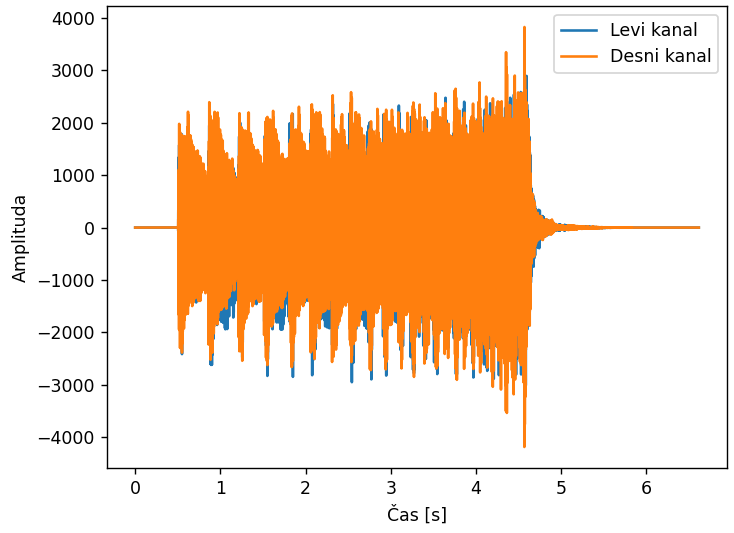
\includegraphics[width=\linewidth]{wave.png}
        \caption{Slika celotnega WAVE posnetka. Glasba se začne okoli 0.5 s in konča okoli 5 s, posnetek pa je malo daljši od 6 s.}
        \label{fig:sub1}
    \end{subfigure}%
    \hspace{1em}%
    \begin{subfigure}[t]{.45\textwidth}
        \centering
        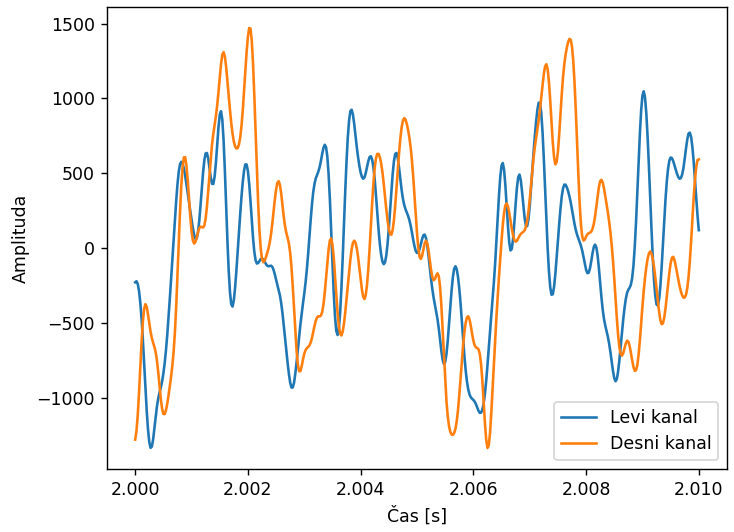
\includegraphics[width=\linewidth]{wave_zoom.png}
        \caption{Izrezani 10 ms del iz posnetka levo. Na sliki je prikazano, da je vsebina WAVE datoteke valovna oblika posnetega signala.}
        \label{fig:sub2}
    \end{subfigure}
\caption{Prikaz WAVE datoteke posnetka \\ AkPnBcht/ISOL/TR1/MAPS\_ISOL\_TR1\_F\_S0\_M53\_AkPnBcht.wav.}
\label{fig:wave}
\end{figure}

MIDI (\en\ Musical Instrument Digital Interface) je standardni komunikacijski protokol za komunikacijo med elektronskimi inštrumenti, računalniki in glasbenimi napravami za namene snemanja, predvajanja in urejanja glasbe.
MIDI ima svoj standardni datotečni zapis (s končnico .mid), kamor se lahko zapišejo skladbe.
Vsaka skladba ima lahko več inštrumentov, ki so označeni z vrsto.
Vsak inštrument vsebuje seznam not, ki jih igra.
Note so označene z začetkom, koncem, višino tona in glasnostjo.
MIDI datoteke so izjemno uporabne, saj omogočajo enostaven prenos, urejanje in predvajanje glasbenih vsebin.
Primer vsebine MIDI datoteke je prikazana na sliki \ref{fig:midi}.

\begin{figure}
    \centering
    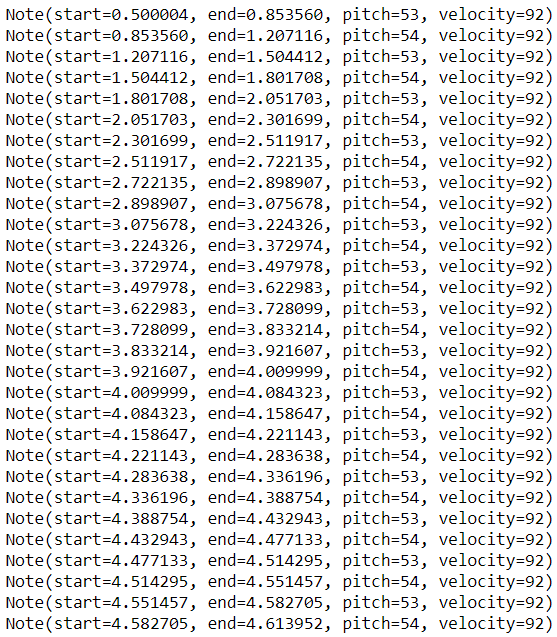
\includegraphics[width=0.5\textwidth]{slike/midi_file.png}
    \caption{Vsebina MIDI datoteke \\ AkPnBcht/ISOL/TR1/MAPS\_ISOL\_TR1\_F\_S0\_M53\_AkPnBcht.mid. Datoteka vsebuje note, vsaka nota ima začetek, konec, višino in glasnost. Pitch označuje višino tona v MIDI številkah. MIDI številki 53 in 54 označujeta tona mali F in mali FIS.}
    \label{fig:midi}
\end{figure}

\section{Spektrogrami}

Transkripcija glasbe je naloga, pri kateri se poskuša ugotoviti, kateri toni so prisotni v določenem delu skladbe.
Ker so toni primarno definirani z njihovo višino ali frekvenco, si pri transkripciji glasbe lahko pomagamo s spektrogrami.
Spektrogram je vizualna predstavitev frekvenčnega prostora signala skozi čas.
Frekvence, ki so prisotne v signalu, lahko dobimo tako, da signal pretvorimo iz časovnega v frekvenčni prostor.
Vendar pretvorbe ne moremo narediti na celotnem signalu naenkrat, saj tako izgubimo časovno komponento.
Rezultat bi bil seznam vseh frekvenc, ki so prisotne v signalu, to pa nam ne koristi pri transkripciji.
Pretvorba se mora tako izvesti nad krajšim delom signala, ki mu pravimo okno.
Velikost okna določa natančnost frekvenčnega prostora.
Preveliko okno pomeni izgube v časovni komponenti, s premajhnim pa ne zaznamo nizkih frekvenc zaradi premajhnega števila vzorcev, zato moramo velikost okna izbrati previdno.
Če okna nato zložimo enega zraven drugega, dobimo sliko frekvenčnega prostora, ki je odvisen od časa.
V nadaljevanju si oglejmo dve najpogostejši pretvorbi iz časovnega v frekvenčni prostor: diskretno Fourierovo transformacijo (\en\ Discreet Fourier Transform -- DFT) in transformacijo s konstantnim Q (\en\ Constant Q Transform -- CQT).

Diskretna Fourierova transformacija je diskretna oblika Fourierove transformacije, ki lahko transformira poljubno neperiodično funkcijo v kombinacijo sinusoid z različnimi frekvencami, fazami in amplitudami.
Naš signal je neperiodična funkcija, zato namesto Fourierove vrste uporabimo Fourierovo transformacijo.
Poleg tega signala nimamo podanega kot funkcijo, ampak kot zajeti kvantizirani vzorec, zato uporabimo DFT.
Pri tem si lahko pomagamo z algoritmom hitra Fourierova transformacija (\en\ Fast Fourier Transform -- FFT), ki predstavlja učinkovito implementacijo DFT s časovno kompleksnostjo $ O(n\,log\,n) $, kjer $ n $ predstavlja število vzorcev v signalu.

Enačba \ref{eq:fft} predstavlja enačbo DFT.
Pri tem v enačbi $ N $ predstavlja število zajetih vzorcev ali velikost okna in $ x_n $ predstavlja zajeti signal ob časih $ k = 0, 1, \dots, N-1 $.
$ X_k $ je kompleksno število, ki predstavlja amplitudo in fazo sinusoid s frekvenco $ k/N $ na časovno enoto, ki je enaka velikosti okna.
Zaloga vrednosti enačbe DFT so tako kompleksna števila.
Amplitudo signala dobimo z izračunom velikosti kompleksnega števila po formuli $ \left|z\right|=\sqrt{Im(z)^{2}+Re(z)^{2}} $.

\begin{equation}
\label{eq:fft}
    X_k = \sum_{n=0}^{N-1}{x_n e^{-i\,2\pi\,n\,k/N}}
\end{equation}

Pri tem smo omejeni z zaznavo frekvenc.
Po Nyquist-Snannonovem teoremu ne moremo zaznati frekvenc, ki so večje od polovične frekvence vzorčenja.
Ker imamo WAVE datoteke, ki so vzorčene pri 44,1 kHz, DFT ne mora zaznati frekvenc, ki so višje od 22,05 kHz.
Najvišji ton na klavirju je C5 (MIDI oznaka C8 ali številka 108) s frekvenco 4186 Hz, kar pomeni, da lahko vse tone klavirja zaznamo.

V praksi se uporablja tudi algoritem kratko-časovna Fourierova transformacija (\en\ Short-Time Fourier Transform -- STFT), ki je različica FFT algoritma.
STFT je narejen za namene raziskovanja, kako se frekvence spreminjajo skozi čas.
Algoritem signal sam razdeli na bloke (okna), ki se lahko prekrivajo med sabo, in nad njimi izvede transformacijo.
Slika primera izhoda STFT algoritma je predstavljena na sliki \ref{fig:spectrogram}(a). Zaradi preglednosti je na sliki \ref{fig:spectrogram}(b) prikazana povečava istega primera spektrograma.

Transformacija s konstantnim Q \cite{brown1991cqt} je podobna DFT z nekaj pomembnimi razlikami.
Algoritem CQT uporabi različno velika okna za zaznavo različno visokih frekvenc, medtem ko ima DFT okna konstantne velikosti.
Za nizke frekvence uporabi daljše okno, kar nam poveča frekvenčno resolucijo, za visoke frekvence pa uporabi krajše okno, kar nam da visoko časovno resolucijo.
S tem algoritem CQT predstavlja dober kompromis med časovno in frekvenčno resolucijo.
Druga razlika je uporaba logaritemske lestvice.
DFT razdeli frekvenčni prostor linearno, medtem ko CQT uporabi logaritemsko lestvico.
Uporaba logaritemske lestvice izhaja iz biološkega vidika zaznavanja zvoka, ki ga zaznavamo logaritemsko.
Če ima osnovni ton frekvenco $ f_{0} $, ima ton, ki je oktavo višje od osnovnega, frekvenco $ f_{1} = 2 f_{0} $, in ton, ki je dve oktavi nad osnovnim, frekvenco $ f_{2} = 2 f_{1} = 4 f_{0} $.
Zaradi tega so višji toni v frekvenčnem prostoru vedno bolj narazen, medtem ko so nižji toni vedno bolj skupaj.
Ko pa jih poslušamo, imamo občutek, da so narazen linearno.
DFT z linearno skalo zato ne razločuje najbolje med nizkimi toni, hkrati pa pušča ogromno prostora med toni z visokimi frekvencami.
CQT izkoristi znanje o relaciji med frekvencami tonov in jih zato izračuna na logaritemski lestvici.
Slika primera izhoda CQT algoritma je na sliki \ref{fig:spectrogram}(c).

\begin{figure}
    \centering
    \begin{subfigure}[t]{.45\textwidth}
        \centering
        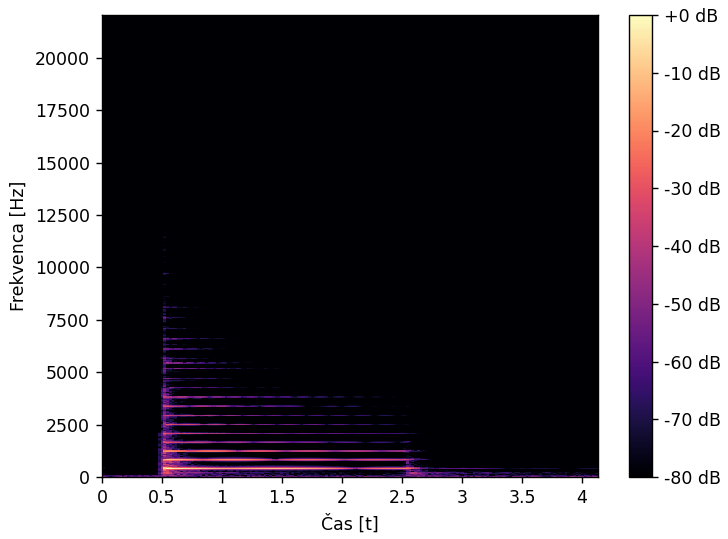
\includegraphics[width=\linewidth]{stft.png}
        \caption{STFT spektrogram tona A1.}
        \label{fig:stft}
    \end{subfigure}%
    \hspace{1em}%
    \begin{subfigure}[t]{.45\textwidth}
        \centering
        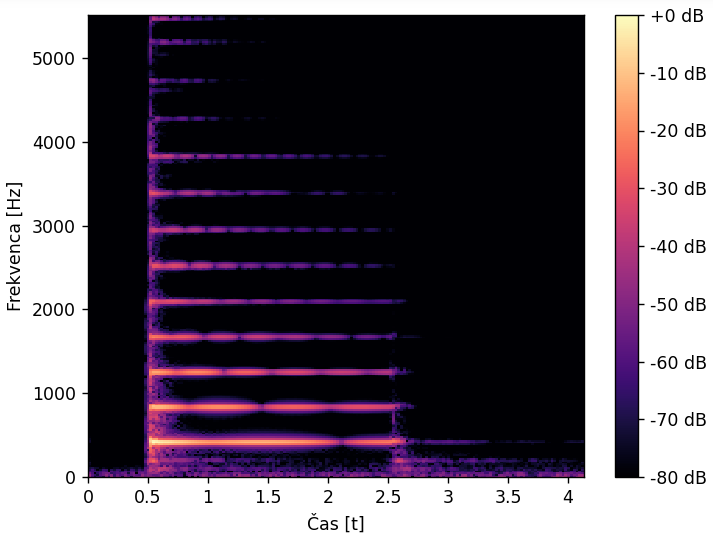
\includegraphics[width=\linewidth]{stft_zoom.png}
        \caption{Povečan STFT spektrogram tona A1.}
        \label{fig:stft_zoom}
    \end{subfigure}
    \begin{subfigure}[t]{.45\textwidth}
        \centering
        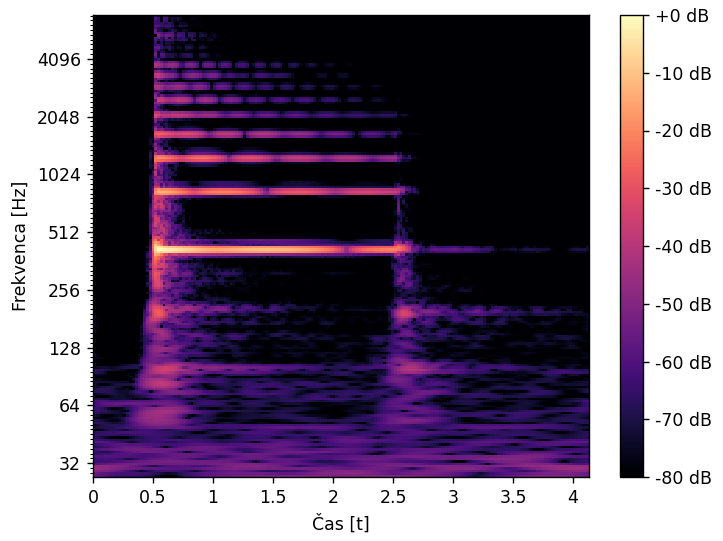
\includegraphics[width=\linewidth]{cqt.png}
        \caption{CQT spektrogram tona A1.}
        \label{fig:cqt}
    \end{subfigure}
    
    \caption{Slike spektrogramov tona A1 s frekvenco 440 Hz. Na sliki levo je primer STFT spektrograma in na sliki desno je povečava slike levo. Na sliki spodaj je primer CQT spektrograma. CQT spektrogram ima logaritemsko skalo, medtem ko je skala STFT spektrograma linearna. Zato se na CQT spektrogramu lažje vidi prisotne frekvence, medtem ko so na STFT spektrogramu (levo) zelo nepregledne. Sliki levo in spodaj sta neposredna izhoda algoritmov STFT in CQT in nista spremenjeni, frekvenčni osi pa sta samo označeni s pravilnimi vrednostmi.}
    \label{fig:spectrogram}
\end{figure}

\section{Modeli učenja}

Za avtomatsko transkripcijo glasbe smo implementirali modele z nevronskimi mrežami in konvolucijskimi nevronskimi mrežami.

Nevronska mreža je model strojnega učenja, ki uporablja več plasti celic ali nevronov, ki so povezani med sabo.
Vsaka NN ima vsaj dve plasti, vhodno in izhodno plast, lahko pa ima tudi vmesne plasti, ki se imenujejo skrite.
Vsaka plast je sestavljena iz več nevronov, vsi nevroni ene plasti imajo za vhod izhode nevronov prejšnje plasti.
Tako dobimo mrežo povezav, ki je zmožna aproksimirati zelo kompleksne relacije/funkcije.

Vsak nevron je definiran kot utežena vsota izhodov prejšnje plasti, nad katerim je izvedena aktivacijska funkcija, kot je to prikazano v enačbi \ref{eq:neuron}.

\begin{equation}
\label{eq:neuron}
    x_{j}^{l} = f\left(\sum_{k=0}^{n_{l-1}}w_{jk}^{l}x_{k}^{l-1} + b_{j}^{l}\right)
\end{equation}

Tu $ x_{j}^{l} $ predstavlja vrednost $ j $-tega nevrona v $ l $-ti plasti, $ \sum_{k=0}^{n_{l-1}}w_{jk}^{l}x_{k}^{l-1} $ predstavlja uteženo vsoto vrednosti nevronov prejšnje plasti, $ b_{j}^{l} $ predstavlja pristranskost (\en\ bias) nevrona $ j $ in $ f $ predstavlja aktivacijsko funkcijo.
Enačba je grafično prikazana na sliki \ref{fig:neuron}.

\begin{figure}
    \centering
    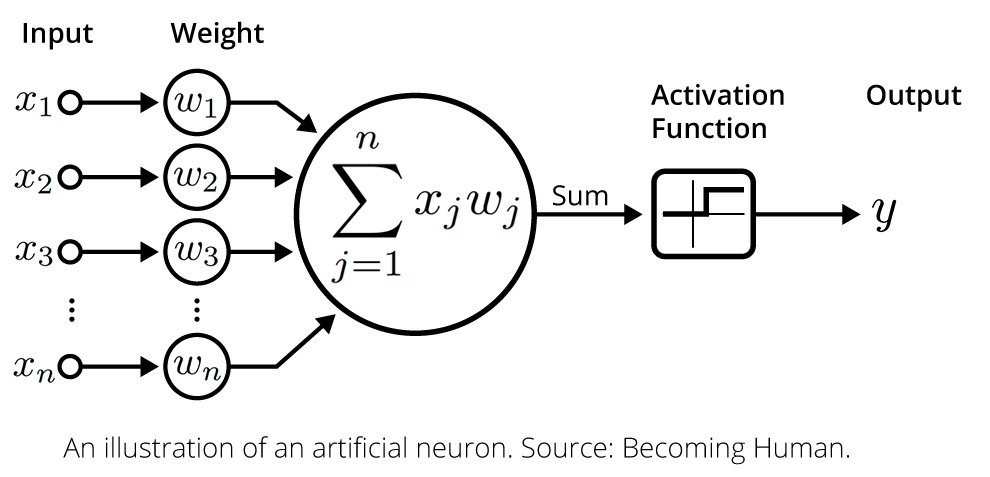
\includegraphics[width=0.5\textwidth]{activation-function.png}
    \caption{Grafični prikaz enačbe nevrona. Vir: https://www.freecodecamp.org/news/deep-learning-neural-networks-explained-in-plain-english/}
    \label{fig:neuron}
\end{figure}

Najpogosteje uporabljene aktivacijske funkcije so ReLU (\en\ Rectified Linear Unit), sigmoidna funkcija (\en\ sigmoid) in hiperbolični tangens (tanh).
ReLU funkcija omeji izhod nevrona na interval $ [0, \infty) $.
Pri tem pozitivne vrednosti pusti pri miru in negativne nastavi na 0.
Zaradi izpuščanja negativnih vrednosti je računsko enostavna, prav tako omogoča hitrejšo konvergenco do lokalnega minimuma funkcije izgube (\en\ loss function).
Sigmoidna funkcija, imenovana tudi logistična funkcija, izhod omeji na interval $ (0, 1) $.
Funkcija je upobna, ko hočemo izhod interpretirati kot verjetnost, in je odvedljiva, kar poenostavi učenje.
Hiperbolični tangens je zelo podoben sigmoidni funkciji, le da izhod omeji na interval $ (-1, 1) $.
Izhode si tako lahko razlagamo kot negativne, nevtralne ali pozitivne.
Ker ima hiperbolični tangens bolj strm odvod kot sigmoidna funkcija, je bolj primeren za hitrejše učenje.

Ker enačba \ref{eq:neuron} velja za vse nevrone v NN, jo lahko zapišemo v matrični obliki v enačbi \ref{eq:nn}.

\begin{equation}
\label{eq:nn}
    X_{l} = f\left(W_{l}X_{l-1} + B_{l}\right)
\end{equation}

V njej je $ X_{l} $ stolpični vektor, ki predstavlja izhod plasti $l$.
$ W_{l} $ je matrika uteži plasti $ l $ in je velikosti $ n_{l-1} \times n_{l} $, kjer $ n_{l} $ predstavlja velikost $ l $-te plasti.
$ B_{l} $ predstavlja stolpični vektor pristranskosti plasti $ l $.
Med matriko $ W_{l} $ in vektorjem $ X_{l-1} $ poteka skalarno množenje.

NN je mogoče učiti zaradi algoritma, ki se imenuje vzvratno razširjanje napake (\en\ backpropagation of error) in uporablja gradientni spust.
Pri učenju NN se najprej pri določenem vhodu izračunajo vrednosti vseh nevronov in končno tudi vrednosti izhodov, ki se nato primerjajo s pravilnimi izhodi.
Iz razlike se nato s pomočjo odvodov izračuna, za koliko je potrebno katere parametre NN spremeniti.
Parametri NN so uteži $ w_{jk}^{l} $ in pristranskosti $ b_{j}^{l} $ vseh nevronov.

Konvolucijska nevronska mreža je mreža, ki je podobna NN z razliko, da implementira konvolucijo.
Konvolucija (\en\ convolution) je matematična operacija med dvema funkcijama, katere izhod je funkcija, ki opisuje, kako je oblika ene funkcije spremenjena z drugo funkcijo.
Pri tem pogosto rečemo, da je druga funkcija filter, ki se izvede na prvi funkciji.

Enačba \ref{eq:conv} je enačba konvolucije. V enačbi je funkcija $ f $ spremenjena s funkcijo $ g $.
Izhod je funkcija $ (f * g) $.
Konvolucija se pogosto uporablja pri obdelavi slik, računalniškem vidu in obdelavi signalov.

\begin{equation}
\label{eq:conv}
    (f * g)(t) = \int_{-\infty}^{\infty}f(\tau)g(t-\tau)\,d\tau
\end{equation}

CNN so NN s konvolucijskimi plastmi.
Pri tem so povezave med plastmi lokalne in deljene med nevroni.
Tako je vsak nevron naslednje plasti povezan le z nekaj nevroni prejšnje plasti.

Pri CNN so v uporabi tudi podvzorčne (\en\ subsampling, downsampling, pooling) plasti.
Te zmanjšajo izhod ene konvolucijske plasti pred vhodom v naslednjo plast.
S tem se podatki agregirajo in naslednje plasti dobijo manj podatkov v obdelavo, kar zmanjšuje število parametrov in čas učenja.
Podvzorčenje poteka tako, da se iz določene regije izhoda konvolucijske plasti ohrani ali izračuna le ena številka.
Pogosti podvzorčni plasti sta Max pooling, ki ohrani samo največjo vrednost določene regije, in Average pooling, ki vrne povprečno vrednost določene regije.

\section{Metrike}

Pri strojnem učenju moramo vedeti, kako dober je model po učenju.
Pri tem si pomagamo z metrikami.
Metrike so kvantitativne meritve, s katerimi lahko merimo uspešnost, učinkovitost ali lastnost nečesa.
V našem primeru metrike na naučenih modelih predstavljajo njihovo lastnost uspešnosti pri napovedovanju na še ne videnih podatkih.
Pri tem se najprej določijo osnovne metrike, iz katerih se lahko izračunajo bolj kompleksne: resnično pozitivni (\en\ true positive, TP), resnično negativni (\en\ true negative, TN), lažno pozitivni (\en\ false positive, FP) in lažno negativni (\en\ false negative, FN) primeri.
TP nam predstavlja število primerov, ki so definirani kot pozitivni in jih je model označil za pozitivne.
TN je število negativnih primerov, ki jih je model označil za negativne.
FP in FN so primeri, ki jih je model označil ravno nasprotno, kot pa so v resnici.
Pri strojnem učenju se najpogosteje uporabljajo metrike točnosti (\en\ accuracy), senzitivnosti (\en\ sensitivity) in specifičnosti (\en\ specificity).


Točnost se pogosto uporablja v binarnih klasifikacijskih primerih, kjer imamo pozitivne in negativne primere.
Točnost se izračuna po enačbi \ref{eq:acc}, kjer se število resnično pozitivnih in resnično negativnih primerov deli s številom vseh primerov.
S tem dobimo odstotek, ki nam pove, koliko primerov je model pravilno klasificiral oziroma uvrstil.

\begin{equation}
\label{eq:acc}
    \text{točnost} = \frac{TP+TN}{TP+FP+TN+FN}
\end{equation}

Senzitivnost nam pove, kolikšen odstotek primerov, ki jih je model označil za pozitivne, je res pozitivnih.
Izračuna se po enačbi \ref{eq:sens}, kjer se število resnično pozitivnih primerov deli z vsoto števila resnično pozitivnih in števila lažno negativnih primerov.

\begin{equation}
\label{eq:sens}
    \text{senzitivnost} = \frac{TP}{TP+FN}
\end{equation}

Specifičnost je mera, ki nam pove, kolikšen odstotek primerov, ki jih je model označil za negativne, je res negativnih.
Izračuna se po enačbi \ref{eq:spec}, kjer se število resnično negativnih primerov deli z vsoto števila resnično negativnih in števila lažno pozitivnih primerov.

\begin{equation}
\label{eq:spec}
   \text{specifičnost} = \frac{TN}{TN+FP}
\end{equation}

Če gledamo na problem transkripcije glasbe kot na klasifikacijski problem, lahko vidimo, da je od zgoraj naštetih mer za nas zanimiva samo senzitivnost.
Ker je v skladbah v veliki večini naenkrat prisotnih le nekaj tonov (pozitivni primeri), je tako velika večina primerov negativnih.
Model, ki ne bi napovedoval nič, bi tako dosegel visoko točnost in specifičnost, a nizko senzitivnost.
Za podatke, kjer je pozitivnih primerov malo, in za potrebe diplomske naloge potrebujemo še metrike preciznosti (\en\ percision), priklica (\en\ recall) in F vrednosti (\en\ F-score).

Preciznost se izračuna po enačbi \ref{eq:prec}, kjer se število resnično pozitivnih primerov deli z vsoto števila resnično pozitivnih in števila lažno pozitivnih primerov.

\begin{equation}
\label{eq:prec}
    \text{preciznost} = \frac{TP}{TP+FP}
\end{equation}

Priklic se izračuna po enačbi \ref{eq:rec}, kjer se število resnično pozitivnih primerov deli z vsoto števila resnično pozitivnih in števila lažno negativnih primerov.
Pomembno je poudariti, da imata priklic in senzitivnost enak pomen in enaki formuli, razlika je le v tem, da ime senzitivnost izvira iz področja statistike, medtem ko ime priklic izvira iz področja informatike.

\begin{equation}
\label{eq:rec}
    \text{priklic} = \frac{TP}{TP+FN}
\end{equation}

Preciznost nam tako pove, koliko izbranih elementov je ustreznih, priklic pa, koliko ustreznih elementov je bilo izbranih. Pri tem so izbrani elementi tisti, ki jih je model označil za pozitivne, ustrezni pa tisti, ki so zares pozitivni.

F vrednost je harmonična sredina med preciznostjo in priklicem, izračuna se po enačbi \ref{eq:f}.
Opisuje uspešnost binarne klasifikacije, kjer imamo veliko število negativnih primerov.
V diplomski nalogi smo jo uporabili za splošno uspešnost modela, kjer višja F vrednost pomeni boljši model.

\begin{equation}
\label{eq:f}
    \text{F vrednost} = 2 * \frac{\text{preciznost} * \text{priklic}}{\text{preciznost} + \text{priklic}}
\end{equation}

\chapter{Poskusi}
\label{ch:work}

\section{Podatki in obdelava}
\label{ch:preprocessing}

Pri diplomski nalogi smo uporabili podatkovno zbirko anotiranih klavirskih skladb MAPS (MIDI Aligned Piano Sounds) \cite{maps}.
V zbirki so posneti trije virtualni klavirji (The Grand 2 iz programa Steinberg, Akoustik Piano iz programa Native Instruments in The Black Grand iz programa Sampletekk) in en resnični klavir, disklavir.
Snemani so bili na različnih krajih, kot so cerkev, koncertna dvorana in studio, skupno je tako v zbirki devet različnih kombinacij klavirjev in snemalnih krajev.
Posnetki so shranjeni v WAVE formatu, zraven vsakega je tudi pripadajoča MIDI datoteka.
Posnetki posameznih kombinacij klavirja in snemalnega kraja so razdeljeni še na štiri podmnožice.
Prva je ISOL, ki vsebuje posnetke posameznih dolgih in kratkih tonov ter kromatičnih lestvic.
Druga je RAND, ki vsebuje posnetke akordov z naključnimi toni in različnim številom prisotnih tonov.
Tretja je UCHO, ki vsebuje akorde, ki so pogosto prisotni v glasbi zahodnega sveta.
Zadnja je MUS, ki vsebuje posnetke klasičnih glasbenih del avtorjev, kot so Bach, Chopin, Grieg, Mozzart, Schubert in drugi.
Za učenje modelov smo se odločili, da uporabimo samo podmnožico MUS, saj nas zanima transkripcija pravih skladb in ne posameznih not.
Za razdelitev skladb na učne in testne so Sigtia, Benetos in Dixon v \cite{sigtia2016endtoend} predlagali, da se model uči na sintetiziranih skladbah virtualnih klavirjev in testira na resničnih posnetkih.
Testne skladbe tako pripadajo posnetkom dveh klavirjev, ki sta označena z ENSTDkAm in ENSTDkCl, vsi ostali posnetki so učni.
Tako razdelitev argumentirajo kot smiselno in logično, saj so anotirane skladbe po navadi posnete v nadzorovanem okolju, medtem ko je glasba, ki jo poskušamo transkribirati, posneta v nenadzorovanem in neidealnem okolju.

Pri pregledu zastopanosti not med učnimi MUS skladbami v MAPS zbirki smo opazili neenakomerno porazdelitev prisotnih not, kar je v klasični glasbi običajno, saj ni pogosto slišati zelo visokih ali nizkih tonov.
Porazdelitev je normalna, kjer velika večina not pripada srednji legi.
Povprečen ton je E1 (MIDI ime E4 in številka 64) s frekvenco 329.63 Hz, standardni odklon pa predstavlja 13.50 tonov, kar je ton in pol več kot ena oktava.
S temi podatki lahko vidimo, da približno 95\% vseh not med MUS skladbami v MAPS zbirki predstavlja 44 različnih tonov, kar predstavlja polovico vseh tonov, ki jih je možno zaigrati na klavirju.
Za boljše učenje smo se odločili, da skladbe transponiramo in tako povečamo zastopanosti vseh tonov.
Transpozicija je glasbeni postopek, pri katerem določeno skupino not prestavimo za določeno število tonov višje ali nižje.
Pri tem se ohranita melodija in ritem, spremeni pa se višina tonov, kar povzroči, da slišimo isto melodijo, ki je nižja ali višja.
Vse učne skladbe v MUS smo transponirali za 30 tonov višje in nižje in tako potrojili število učnih skladb. Testnih skladb se nismo dotikali, saj so bile posnete na resničnih klavirjih.
Pri tem smo za generiranje posnetkov uporabili Python knjižnjico {\sf midi2audio} in njen modul {\sf FluidSynth}.
Po transponiranju smo ponovno pregledali porazdelitev not med učnimi podatki, ki je zdaj veliko bolj uniformna. To daje našemu modelu boljše možnosti, da se nauči vseh tonov in ne samo najbolj pogostih. Distribucija not pred in po transpoziciji se vidi na Sliki \ref{fig:note_dist}.

\begin{figure}
    \centering
    \begin{subfigure}{.45\textwidth}
        \centering
        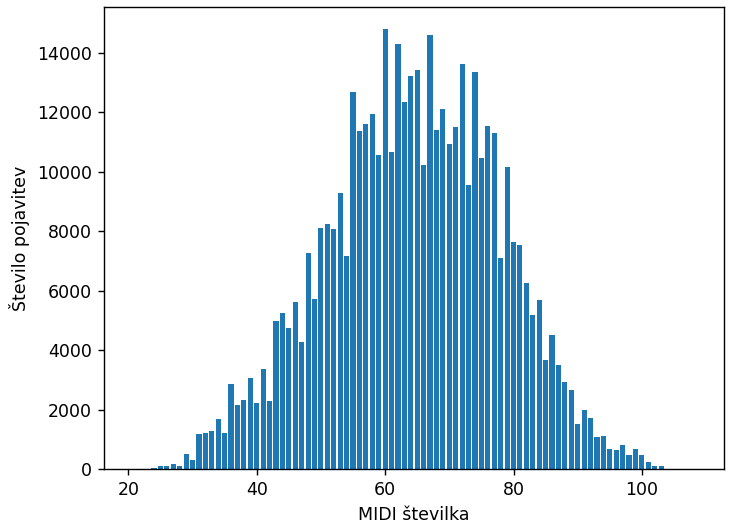
\includegraphics[width=\linewidth]{notes.png}
        \caption{Distribucija not med MUS testnimi skladbami.}
        \label{fig:before}
    \end{subfigure}%
    \hspace{1em}%
    \begin{subfigure}{.45\textwidth}
        \centering
        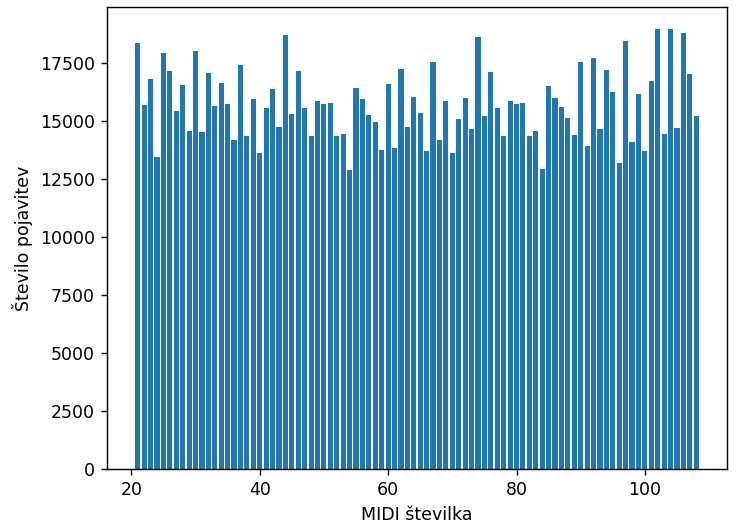
\includegraphics[width=\linewidth]{notes_transposed.png}
        \caption{Distribucija not po transponiranju MUS skladb.}
        \label{fig:after}
    \end{subfigure}
    \caption{Distribucija not pred in po transpoziciji. Slika levo prikazuje distribucijo not med učnimi skladbami v MUS delu MAPS zbirke. Slika desno pikazuje distribucijo not po transpoziciji vseh MUS učnih skladb za 30 tonov navzgor in navzdol. Pred transpozicijo so note porazdeljene normalno, po transpoziciji pa imajo uniformno porazdelitev.}
    \label{fig:note_dist}
\end{figure}

Pri pretvorbi skladb iz WAVE datotek v spektrograme smo uporabili CQT namesto STFT, kot to argumentirajo Sigtia, Benetos in Dixon v \cite{sigtia2016endtoend}.
Za računanje CQT spektrogramov smo si pomagali s Python knjižnico {\sf librosa} \cite{mcfee2015librosa}.
Skladbe smo najprej s povprečenjem kanalov pretvorili v enokanalne.
CQT se je nato izračunal nad 8 oktavami s 24 vrednostmi na oktavo in z velikostjo okna 1024 pri vzorčni frekvenci 44,1 kHz, kar je pomenilo, da je bilo vsako okno dolgo 43,07 ms.
Najnižja frekvenca CQT algoritma je bila nastavljena na 27,5 Hz, kar ustreza tonu A subkontra (MIDI ime A0 in številka 21), ki je najnižji ton na klasičnem klavirju.
Dobljeni spektrogram je tako imel 192 vrstic, ki so predstavljale frekvence tonov.

Normalizacija spektrogramov je potekala na dva načina.
Prvi način je standardizacija.
Izračunali smo 192 povprečnih vrednosti in standardnih odklonov za vsako vrstico posebej nad vsemi spektrogrami, ki so pripadali učni množici.
Nato smo vsem spektrogramom odšteli vektor povprečnih vrednosti in jih delili s standardnimi odkloni.
Standardizacija nam da spektrograme, na katerih se posamezni toni veliko bolje vidijo, vendar pa je ta postopek zelo odvisen od podatkov, ki jih imamo na voljo.
Primer standardiziranega spektrograma je na sliki \ref{fig:normalization}(a).
Drugi način je logaritemska kompresija, ki jo predlagajo Choi in ostali v \cite{choi2021comparison} ter Bőck in Schedl v \cite{bock2012rnn} in je neodvisna od podatkov.
Pri logaritemski kompresiji smo izračunali logaritem spektrograma, ki smo mu prišteli majhno konstanto zaradi preprečevanja računskih napak ($ kompresija = log(spektrogram + \epsilon) $).
Choi in ostali argumentirajo uporabo logaritemske kompresije zaradi človeške zaznave glasnosti, ki je logaritemska in ne linearna \cite{moore2012psy}.
Prav tako so pokazali, da so modeli, učeni na logaritemsko kompresiranih podatkih, boljši.
Primer logaritemsko kompresiranega spektrograma je na Sliki \ref{fig:normalization}(b).

\begin{figure}
    \centering
    \begin{subfigure}[t]{.45\textwidth}
        \centering
        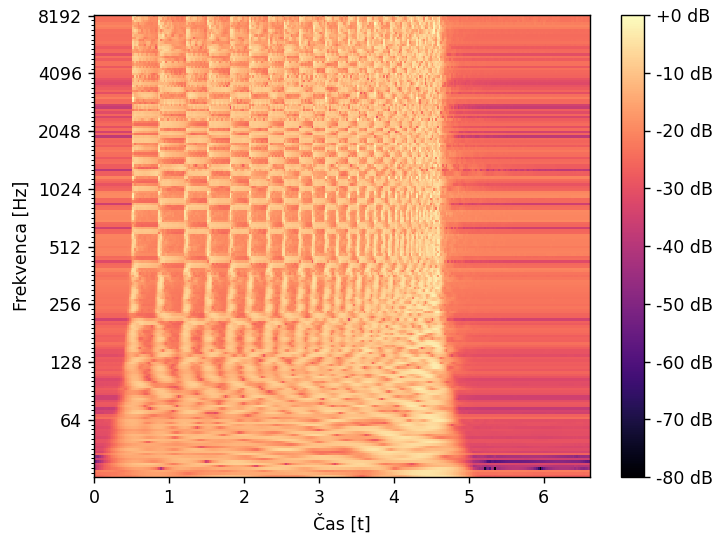
\includegraphics[width=\linewidth]{cqt_z.png}
        \caption{Standardiziran CQT spektrogram.}
        \label{fig:z}
    \end{subfigure}%
    \hspace{1em}%
    \begin{subfigure}[t]{.45\textwidth}
        \centering
        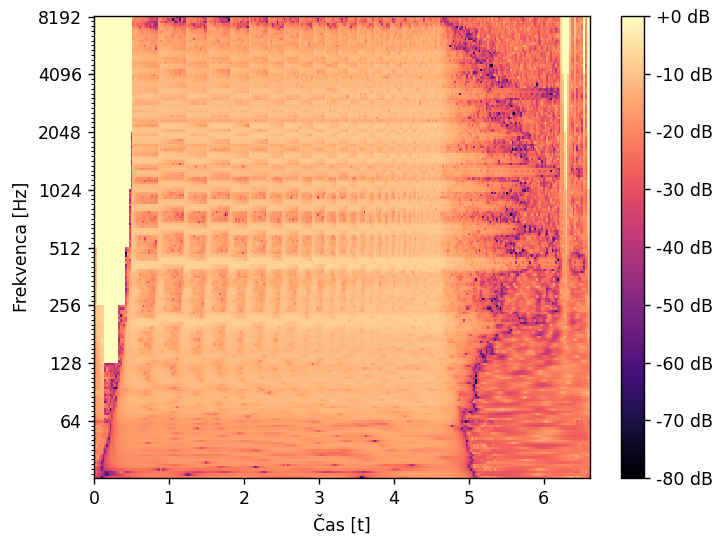
\includegraphics[width=\linewidth]{cqt_log.png}
        \caption{Logaritemsko kompresiran CQT spektrogram.}
        \label{fig:log}
    \end{subfigure}
    \caption{Normalizirana CQT spektrograma. Na sliki levo je standardiziran spektrogram, na sliki desno pa logaritemsko kompresiran CQT spektrogram. Spektrograma na sliki sta nastala iz posnetka AkPnBcht/ISOL/TR1/MAPS\_ISOL\_TR1\_F\_S0\_M53\_AkPnBcht.wav.}
    \label{fig:normalization}
\end{figure}

MIDI datoteke so služile kot ustrezen izhod za skladbe, vendar jih je bilo potrebno spraviti v ustrezno obliko.
Podobno kot WAVE datoteke so bile pretvorjene v spektrograme, vendar na drugačen način.
S pomočjo Python knjižnjice {\sf pretty\_midi} \cite{raffael2014pretty_midi} smo prebrali vse note v MIDI datotekah in njihovo prisotnost označili v binarnih matrikah, ki so prevzele vlogo izhodnih spektrogramov.
Matrike so imele 88 vrstic in toliko stolpcev, kot jih je imel spektrogram pripadajočega WAVE posnetka.
Pri tem smo upoštevali resolucijo spektrogramov, ki je bila 43,07 ms, in z isto frekvenco vzorčili prisotnosti tonov v MIDI datotekah.
Primer MIDI spektrograma je na Sliki \ref{fig:midi_spec}.

\begin{figure}
    \centering
    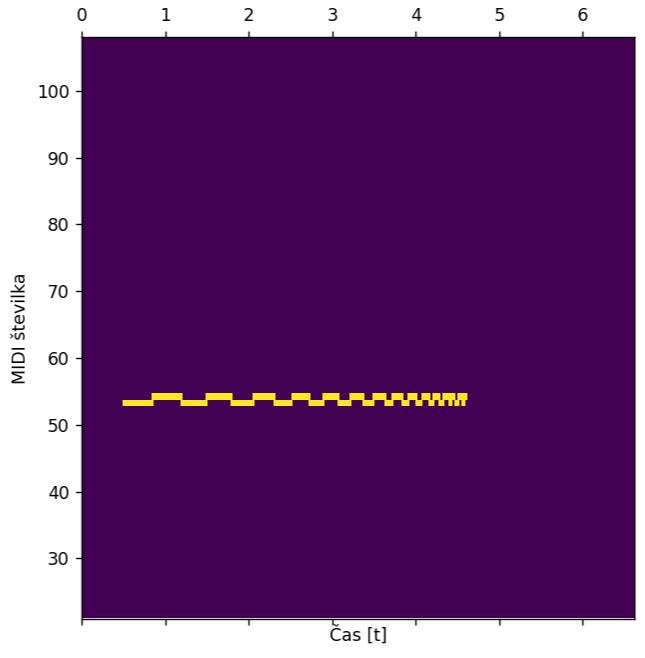
\includegraphics[width=0.5\textwidth]{midi_spec.png}
    \caption{Spektrogram, narejen iz MIDI datoteke \\ AkPnBcht/ISOL/TR1/MAPS\_ISOL\_TR1\_F\_S0\_M53\_AkPnBcht.mid. Na njem je prikazano, kaj je zaigrano na pripadajočem WAVE posnetku.}
    \label{fig:midi_spec}
\end{figure}

\section{Arhitekture nevronskih mrež}

Pri diplomski nalogi smo se osredotočili na raziskovanje, kako velikosti navadnih in konvolucijskih modelov vplivajo na rezultate.
Pri grajenju modelov smo si pomagali s Pyhton knjižnicama {\sf TensorFlow} \cite{tensorflow2015whitepaper} in {\sf Keras}.

Vhod modela je bil del spektrograma, visok 192 in širok 5 celic, kar predstavlja 215,35 ms časovni interval.
Višina je enaka izhodu CQT algoritma, širina 5 pa je okno, ki predstavlja kontekst določenega dela spektrograma v času.
Izhod modela je vektor 88 vrednosti, ki so zaradi logistične aktivacijske funkcije omejene na interval $ (0, 1) $, kjer vrednost 1 pomeni pritisnjeno klavirsko tipko in vrednost 0 nepritisnjeno tipko.
Interval je odprt in zato vrednosti 0 in 1 nista možni, lahko pa si ga razlagamo kot verjetnost, da je določena tipka pritisnjena.
Model napoveduje pritisnjene tipke srednjega (tretjega) stolpca izseka spektrograma. Primer izhoda modela skupaj z resničnim izhodom je prikazan na sliki \ref{fig:output}.

\begin{figure}
    \centering
    \begin{subfigure}{.9\textwidth}
        \centering
        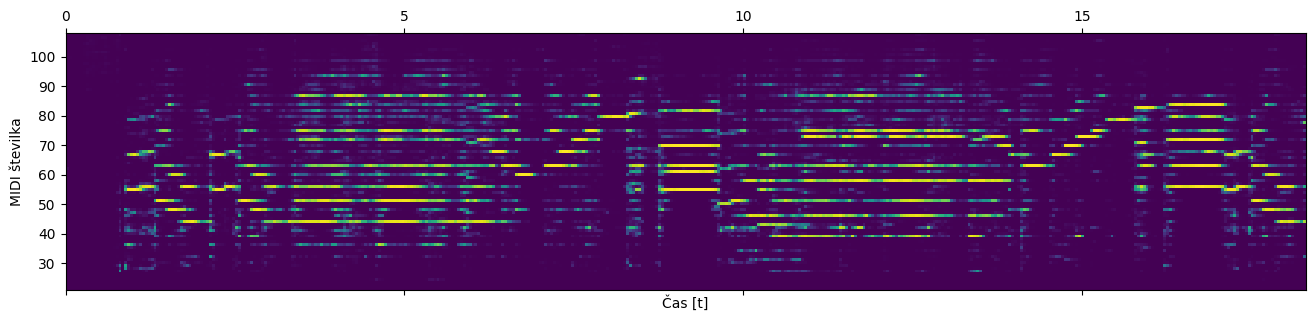
\includegraphics[width=\linewidth]{output.png}
        \caption{Primer izhoda modela. Izhodi so vrednosti na intervalu $ (0, 1) $ in si jih razlagamo kot verjetnost, da je določena tipka na klavirju ob določenem času pritisnjena.}
        \label{fig:out}
    \end{subfigure}
    \begin{subfigure}{.9\textwidth}
        \centering
        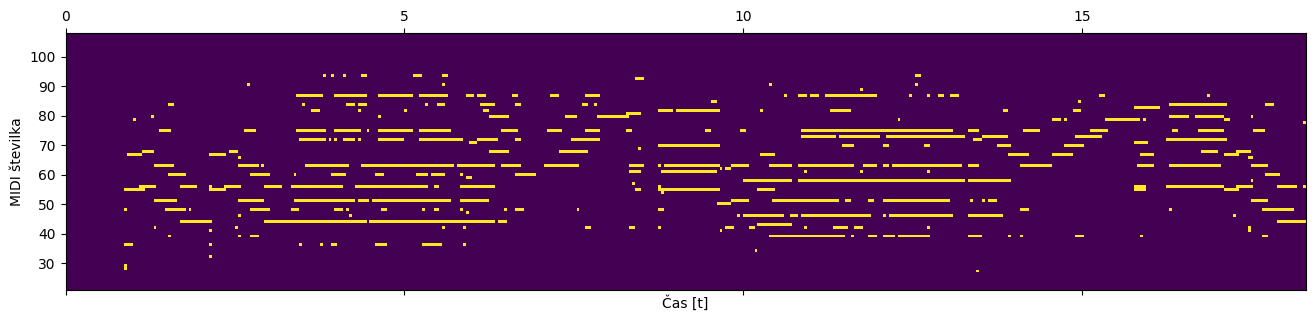
\includegraphics[width=\linewidth]{output_threshold.png}
        \caption{Izhod modela, binariziran s pragom 0,5. Rezultat je izhod, ki ga je mogoče primerjati z resničnim spektrogramom, narejenim iz MIDI datoteke.}
        \label{fig:out_thresh}
    \end{subfigure}
    \begin{subfigure}{.9\textwidth}
        \centering
        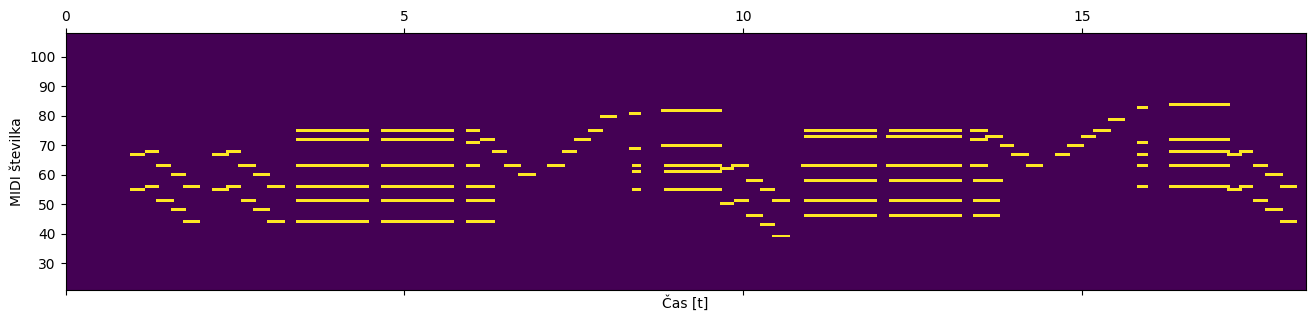
\includegraphics[width=\linewidth]{output_true.png}
        \caption{Resnični izhod modela, imenovan tudi spektrogram iz MIDI datoteke. Na njem se vidi, kaj je dejansko zaigrano.}
        \label{fig:out_real}
    \end{subfigure}
    \caption{Primer izhoda modela za posnetek ENSTDkAm/MUS/MAPS\_MUS-schub\_d760\_3\_ENSTDkAm.wav. \\ Na zgornji sliki so eden zraven drugega zloženi izhodni vektorji modela. Na sredinski sliki je isti izhod binariziran s pragom 0,5. Tako predelani izhod se nato primerja z resničnim spektrogramom, narejenim iz pripadajoče MIDI datoteke, ki je na spodnji sliki.}
    \label{fig:output}
\end{figure}

Pri grajenju modelov smo uporabili Dropout \cite{nitish2014dropout}, ki je tehnika regularizacije za nevronske mreže.
Pri vzvratnem razširjanju napake z Dropoutom se naključne povezave ne upoštevajo, kar omogoča, da se model ne prilagodi preveč učnim podatkom.

Pri opisovanju arhitektur smo zaradi preglednosti izpustili Dropout in MaxPool plasti ter izhodno plast.
Vsi modeli imajo med vsemi plastmi Dropout plasti z verjetnostjo neupoštevanja 10 \%.
Za vsako konvolucijsko plastjo je MaxPool plast s filtrom višine 2 in širine 1.
Izhodna plast modelov je vedno sestavljena iz 88 nevronov in ima logistično aktivacijsko funkcijo, medtem ko imajo vse druge plasti ReLU aktivacijsko funkcijo.
Pri učenju smo uporabili Adam optimizator \cite{kingma2017adam} s stopnjo učenja 0,0006 in binarno entropijsko funkcijo izgube (\en\ Binary Cross--entropy loss funciton).
Pri modelih smo merili preciznost in priklic.
V začetnih poskusih smo opazili, da je priklic vedno veliko nižji od preciznosti, zato smo nastavili priklic kot ciljno metriko pri učenju.
Vsi modeli so se najprej učili 10 prehodov, nato pa so se učili do 200 prehodov, vendar se je učenje prekinilo, če se priklic modela ni izboljšal v 10 prehodih.

Zgradili smo modele štirih različnih arhitektur, ki se primarno razlikujejo po številu in vrsti skritih plasti.
Arhitektura A ima eno konvolucijsko plast, arhitektura B ima dve konvolucijski plasti, arhitektura C ima eno konvolucijsko plast in eno polno povezano plast in arhitektura D ima dve konvolucijski plasti in eno polno povezano plast.
Za vsako arhitekturo smo naredili več različnih modelov, ki so imeli različno število filtrov in nevronov v plasteh.

Velikosti posameznih plasti so zraven imena modelov in njihovega števila parametrov za arhitekture A, B, C in D predstavljene v tabeli \ref{tab:arhAll}.
Pri tem so konvolucijske plasti označene s ''Conv $ n $'', kjer je $ n $ številka plasti, in imajo obliko ''$ \text{štFiltrov} \times (\text{višinaFiltra}, \text{širinaFiltra}) $'', kjer je štFiltrov število filtrov v plasti, (višinaFiltra, širinaFiltra) pa zapis velikosti filtra.
Polno povezane plasti so označene z ''Dense $ n $'', kjer je $ n $ številka plasti, in imajo podano samo število nevronov v plasti.

Velikosti posameznih plasti arhitektur smo izbirali tako, da grajeni modeli pokrivajo čim večji razpon števila parametrov.

\begin{table}[]
    \centering
    \begin{tabular}{c|c|c|c|c}
        Oznaka & Conv 1 & Conv 2 & Dense 3 & Št. parametrov \\
		\hline
        A1 & $ 8 \times (24, 3) $ & -- & -- & 178.080 \\
        A2 & $ 16 \times (24, 3) $ & -- & -- & 356.072 \\
        A3 & $ 24 \times (24, 3) $ & -- & -- & 534.064 \\
		\hline
		B1 & $ 8\times (24, 3) $ & $ 16 \times (12, 3) $ & -- & 55.984 \\
        B2 & $ 16\times (24, 3) $ & $ 32 \times (12, 3) $ & -- & 121.096 \\
        B2 & $ 32\times (24, 3) $ & $ 64 \times (12, 3) $ & -- & 278.968 \\
        \hline
        C1 & $ 8 \times (24, 3) $ & -- & 256 & 1.056.232 \\
        C2 & $ 16 \times (24, 3) $ & -- & 384 & 2.358.448 \\
        C3 & $ 32 \times (24, 3) $ & -- & 384 & 3.133.176 \\
        C4 & $ 32 \times (24, 3) $ & -- & 512 & 4.176.760 \\
		\hline
        D1 & $ 24 \times (24, 3) $ & $ 48 \times (12, 3) $ & 384 & 741.088 \\
        D2 & $ 32 \times (24, 3) $ & $ 64 \times (12, 3) $ & 512 & 1.301.432 \\
        D3 & $ 40 \times (24, 3) $ & $ 96 \times (12, 3) $ & 512 & 1.956.384 \\
    \end{tabular}
    \caption{Hiperparametri in oblike posameznih arhitektur. Arhitektura A ima eno konvolucijsko plast, arhitektura B ima dve konvolucijske plasti, arhitektura C ima eno konvolucijsko plast in eno polno povezano plast in arhitektura D ima dve konvolucijski plasti in eno polno povezano plast.}
    \label{tab:arhAll}
\end{table}


\chapter{Rezultati}
\label{ch:results}

Vsako izmed opisanih arhitektur A, B, C in D smo učili posebej na standardiziranih in posebej na logaritemsko kompresiranih spektrogramih.
Pri tem smo za vsako arhitekturo naučili pet modelov, da smo dobili bolj natančne rezultate o metrikah posamezne arhitekture.
Vse skupaj je bilo naučenih 130 modelov.
Rezultati so predstavljeni v tabeli \ref{tab:results}, kjer posamezne številke predstavljajo povprečno metriko petih učenih modelov.
Rezultati modelov, učenih na standardiziranih spektrogramih, so v stolpcih, označenih s stan (v nadaljevanju: stan modeli), rezultati modelov, učenih na logaritemsko kompresiranih spektrogramih, pa so v stolpcih, označeni z log (v nadaljevanju: log modeli).

\begin{table}[]
    \centering
    \begin{tabular}{c|cc|cc|cc|cc}
         & \multicolumn{2}{c|}{napaka} & \multicolumn{2}{c|}{preciznost} & \multicolumn{2}{c|}{priklic} & \multicolumn{2}{c}{F vrednost} \\
        oznaka & stan & log & stan & log & stan & log & stan & log \\
        \hline
        A1 & 0,0809 & 0,0813 & 0,688 & 0,759 & 0,581 & 0,672 & 0,629 & 0,713 \\
        A2 & 0,0875 & 0,0857 & 0,673 & 0,724 & 0,600 & 0,682 & 0,634 & 0,702 \\
        A3 & 0,0937 & 0,0842 & 0,673 & 0,746 & 0,599 & 0,675 & 0,634 & 0,709 \\
        \hline
        B1 & 0,0694 & 0,0781 & 0,708 & \textbf{0,782} & 0,590 & 0,657 & 0,644 & 0,714 \\
        B2 & \textbf{0,0688} & 0,0774 & \textbf{0,723} & 0,763 & 0,602 & 0,690 & 0,657 & 0,725 \\
        B3 & 0,0690 & 0,0785 & 0,713 & 0,754 & \textbf{0,614} & 0,699 & 0,659 & 0,725 \\
        \hline
        C1 & 0,0939 & 0,0864 & 0,672 & 0,713 & 0,592 & 0,701 & 0,630 & 0,707 \\
        C2 & 0,106 & 0,0941 & 0,666 & 0,683 & 0,596 & 0,713 & 0,629 & 0,697 \\
        C3 & 0,108 & 0,0919 & 0,668 & 0,703 & 0,593 & 0,705 & 0,628 & 0,704 \\
        C4 & 0,118 & 0,0989 & 0,654 & 0,683 & 0,598 & \textbf{0,714} & 0,625 & 0,698 \\
        \hline
        D1 & 0,0701 & \textbf{0,0771} & \textbf{0,723} & 0,756 & 0,609 & 0,709 & \textbf{0,661} & 0,732 \\
        D2 & 0,0738 & 0,0781 & 0,712 & 0,754 & 0,609 & 0,713 & 0,657 & \textbf{0,733} \\
        D3 & 0,0771 & 0,0797 & 0,711 & 0,755 & 0,612 & 0,713 & 0,657 & \textbf{0,733} \\
    \end{tabular}
    \caption{Povprečni rezultati modelov posameznih arhitektur. Stan modeli so v vseh primerih slabši od log modelov. S \textbf{krepko} so označeni najboljši rezultati modelov po posameznih metrikah.}
    \label{tab:results}
\end{table}

Med rezultati se vidi, da imajo log modeli višjo preciznost, priklic in F vrednost.
Pri tem je preciznost log modelov v povprečju višja za 0,0454, priklic za 0,0962 in F vrednost za 0,0728 od stan modelov.
Stan modeli imajo manjšo napako, ta je v povprečju manjša za 0,00199 od napake log modelov.

Razlike med arhitekturami so minimalne, a prisotne.
Najbolj uspešni so modeli arhitekture D s povprečno F vrednostjo 0,696.
Sledijo jim modeli arhitekture B s povprečno F vrednostjo 0,687.
Tretji najuspešnejši modeli pripadajo arhitekturi A s povprečno F vrednostjo 0,670.
Najslabši so modeli arhitekture C, ki imajo povprečno F vrednost 0,665.

Med vsemi modeli sta arhitekturi B in D dosegali najnižje napake na testnih skladbah.
Arhitektura B je imela tudi najvišjo preciznost izmed vseh arhitektur.
Pri priklicu sta najboljši rezultat dosegli arhitekturi B in C.
Najvišjo F vrednost je dosegla arhitektura D.

Razlike med modeli posameznih arhitektur so grafično prikazane in predstavljene na naslednjih slikah, kjer so s polno črto označeni log modeli in s črtkano črto stan modeli.
Slika \ref{fig:loss} prikazuje napake na testnih skladbah.
Pri vseh arhitekturah napaka z velikostjo modela narašča.
Pri arhitekturah B in D imajo stan modeli nižjo napako kot log modeli.
Slika \ref{fig:precision} prikazuje preciznost.
Pri vseh arhitekturah preciznost pada z velikostjo, stan modeli pa imajo vedno slabšo preciznost kot log modeli.
Slika \ref{fig:recall} prikazuje priklic, ki narašča z velikostjo modela. Tudi tu so log modeli vedno boljši od stan modelov.
Slika \ref{fig:fscore} prikazuje F vrednost, za katero izgleda, da pri arhitekturah A in C pada in pri arhitekturah B in D raste s številom parametrov. Log modeli imajo vedno višjo F vrednost kot stan modeli.

\begin{figure}
    \centering
    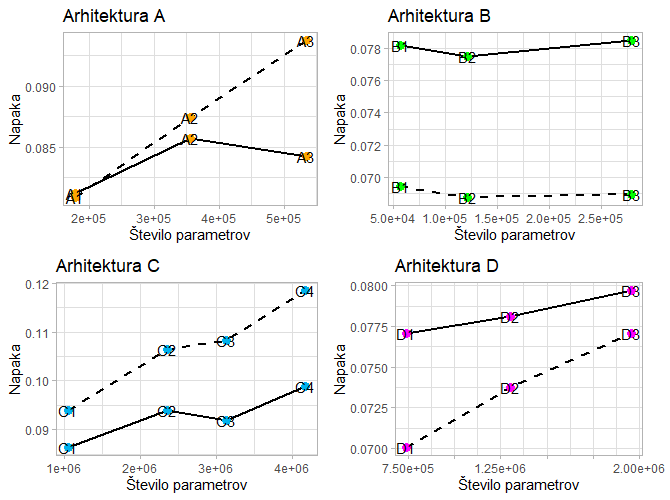
\includegraphics[width=\textwidth]{loss.png}
    \caption{Prikaz funkcije napake po modelih posameznih arhitektur. S polno črto so označeni log modeli in s črtkano stan modeli. Najvišjo napako ima arhitektura C. V večini arhitektur napaka modela narašča z njegovo velikostjo.}
    \label{fig:loss}
\end{figure}

\begin{figure}
    \centering
    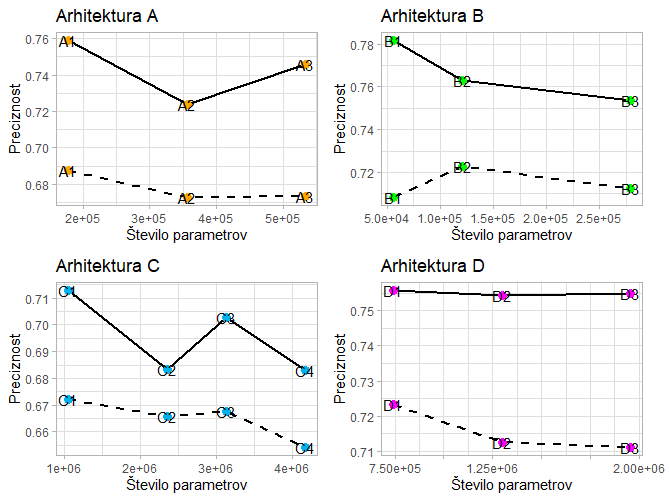
\includegraphics[width=\textwidth]{precision.png}
    \caption{Prikaz preciznosti po modelih posameznih arhitektur. V splošnem preciznost pada z velikostjo modela.}
    \label{fig:precision}
\end{figure}

\begin{figure}
    \centering
    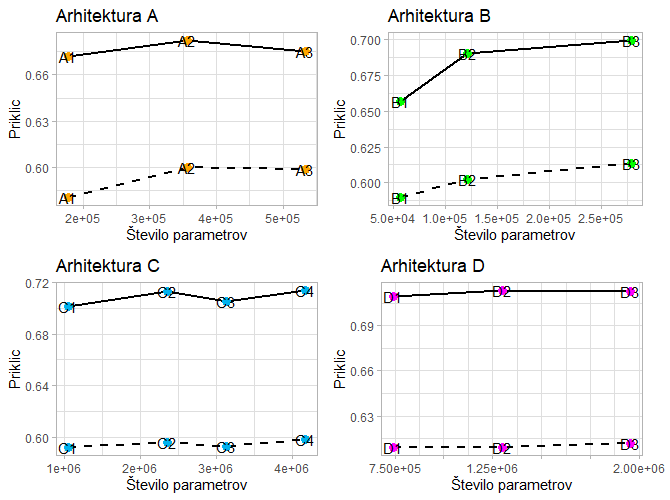
\includegraphics[width=\textwidth]{recall.png}
    \caption{Prikaz priklica po modelih posameznih arhitektur. Priklic narašča z velikostjo modela, kar je po vsej verjetnosti posledica tega, da je priklic ciljna spremenljivka pri učenju.}
    \label{fig:recall}
\end{figure}

\begin{figure}
    \centering
    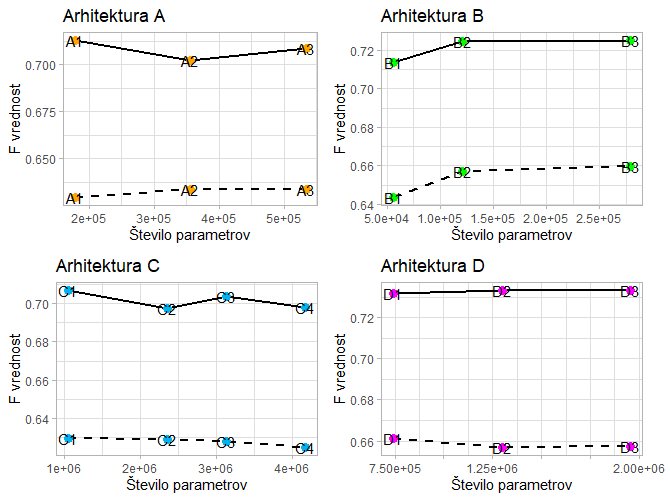
\includegraphics[width=\textwidth]{fscore.png}
    \caption{Prikaz F vrednosti po modelih posameznih arhitektur. Log modeli so konstantno boljši od stan modelov za približno 0,05.}
    \label{fig:fscore}
\end{figure}

Pri učenju modelov smo merili tudi čas prehodov. V tabeli \ref{tab:times} so predstavljeni časi povprečnega prehoda za posamezne modele in arhitekture.
Modeli so bili učeni na grafični kartici NVIDIA Quadro RTX 5000.
Vsi časi so v sekundah.

\begin{table}[]
    \centering
    \begin{tabular}{c|c|c}
        oznaka & stan & log \\
		\hline
        A1 & 111.50 & 110.71 \\
		A2 & 127.19 & 115.14 \\
		A3 & 127.75 & 123.83 \\
		\hline
		B1 & 136.31 & 133.30 \\
		B2 & 136.20 & 136.51 \\
		B3 & 190.40 & 181.23 \\
    \end{tabular}
    \hspace{1em}
    \begin{tabular}{c|c|c}
        oznaka & stan & log \\
		\hline
		C1 & 127.66 & 124.64 \\
		C2 & 136.22 & 143.73 \\
		C3 & 152.08 & 163.16 \\
		C4 & 159.85 & 170.04 \\
		\hline
		D1 & 166.37 & 161.87 \\
		D2 & 189.94 & 200.54 \\
		D3 & 250.31 & 264.48 \\
    \end{tabular}
    \caption{Povprečni časi enega prehoda pri učenju. Vsi časi so v sekundah [s]. Najdaljši prehod ima arhitektura D, ki ima dve konvolucijski plasti. Čeprav ima arhitektura C največ parametrov, nima najdaljšega časa prehoda.}
    \label{tab:times}
\end{table}

Arhitektura A je imela najkrajše prehode, kar je smiselno, saj ima najmanjše modele.
Arhitektura D ima najdaljše prehode pri učenju.
Arhitektura C ima dolžino prehodov bližje arhitekturi A kot D, kar nam pove, da čas učenja ni odvisen samo od števila parametrov, ampak tudi od oblike modela.
Med posameznimi arhitekturami pa so rezultati pričakovani.
Pri isti arhitekturi se pri večjem številu parametrov čas enega prehoda podaljša.

Rezultate naših najboljših modelov posameznih arhitektur lahko primerjamo z modeli drugih raziskovalcev, ki so veljali za State-of-the-Art ali dobre modele s področja okvirne avtomatske transkripcije glasbe.
Vsi primerjani modeli so bili učeni na podatkovni zbirki MAPS in so imeli enako razdelitev skladb na učne in testne.
Za primerjavo smo vzeli model ConvNet, ki so ga predstavili Sigtia in ostali v \cite{sigtia2016endtoend} leta 2016, model AllConv, ki so ga predstavili Kelz in ostali leta 2016 v \cite{kelz2016potential}, model OnsetAndFrames, ki so ga naredili Hawthorne in ostali v \cite{hawthorne2018onsets} leta 2018, in model ADSRNet, ki so ga predstavili Kelz in ostali v \cite{kelz2019deep} leta 2019.

Model ConvNet ima dve konvolucijski, dve polno povezani plasti in izhodno plast.
Skupno ima 1.789.438  parametrov.
Model AllConv ima 7 konvolucijskih plasti in izhodno plast.
Kljub številčnim plastem ima samo 284.544 parametrov.
Model OnsetAndFrames pa je mnogo kompleksnejši, saj vsebuje detektor za začetke not in okvirni detektor.
Njegova arhitektura je podrobneje predstavljena v njegovem članku.
Uradna številka parametrov ni znana, Kwon in ostali v \cite{kwon2020polyphonic} pa ocenjujejo, da ima model med 18.3 in 23.5 milijonov parametrov.
Model ADSRNet je sestavljen iz šestih konvolucijskih in treh izhodnih plasti.
Izhodne plasti služijo za napoved začetka, sredine in konca določene note.
Model ima 326.394 parametrov.

Rezultate smo primerjali v tabeli \ref{tab:comparison}.
Vsi naši modeli so boljši od modela AllConv.
Po uspešnosti mu je najbližji C4, a ima ta 14-krat več parametrov.
Modela B2 in D2 sta boljša od ConvNet, pri tem ima B2 14-krat manj parametrov.
D2 in ConvNet sta si po številu parametrov bližje, a jih ima D2 tretjino manj.
ADSRNet in OnsetAndFrames pa sta mnogo boljša.
OnsetAndFrames dosega skupno najboljše rezultate, kar je po vsej verjetnosti posledica njegove velikosti in kompleksnosti.
ADSRNet je veliko manjši in po parametrih primerljiv z modelom A2, a ima veliko več konvolucijskih plasti, ki zmanjšajo število parametrov in so bolj primerne za učenje iz spektrogramov kot polno povezane plasti.

\begin{table}[]
    \centering
    \begin{tabular}{c|c|c|c|c}
        oznaka & Št parametrov & preciznost & priklic & F vrednost \\
        \hline
        A1 & 178.080 & 0,759 & 0,672 & 0,713 \\
        B2 & 121.096 & 0,763 & 0,690 & 0,725 \\
        C4 & 4.176.760 & 0,683 & 0,714 & 0,698 \\
        D2 & 1.301.432 & 0,755 & 0,713 & 0,733 \\
        \hline
        ConvNet \cite{sigtia2016endtoend} & 1.789.438 & 0.720 & 0,733 & 0,722 \\
        AllConv \cite{kelz2016potential} & 284.544 & 0,765 & 0,635 & 0,694 \\
        ADSRNet \cite{kelz2019deep} & 326.394 & 0,907 & 0,679 & 0,772 \\
        OnsetAndFrames \cite{hawthorne2018onsets} & 18,3-23,5 mio. & 0,885 & 0,709 & 0,783 \\
    \end{tabular}
    \caption{Log modeli primerjani z modeli drugih avtorjev. Modeli so boljši od modela AllConv iz leta 2016 in primerljivi z modelom ConvNet iz leta 2016, ki ima od ostalih najmanj kompleksno arhitekturo. ADSRNet in OnsetAndFrames dosegata veliko višje rezultate.}
    \label{tab:comparison}
\end{table}



\chapter{Zaključek}
\label{ch:discussion}

Iz grafov rezultatov vidimo, da preciznost pada in priklic narašča z velikostjo modela.
To je po vsej verjetnosti posledica dejstva, da je priklic glavna metrika pri učenju.
Večji modeli lahko dosegajo boljše rezultate in na grafih priklica je to tudi prikazano.
Vendar splošno uspešnost modela merimo z F vrednostjo, ki pa je nismo mogli imeti za ciljno, saj bi isto F vrednost lahko model dosegel z različnim naborom preciznosti in priklica.

Iz rezultatov vidimo, da imajo višje F vrednosti arhitekture z več konvolucijskimi plastmi.
Taki arhitekturi sta B in D.
D ima za razliko od arhitekture B še eno dodatno navadno plast, kar ji očitno da prednost pred arhitekturo B.
Stvar se ravno obrne pri arhitekturama A in C.
Obe imata samo eno konvolucijsko plast, arhitektura C ima za njo še eno navadno plast.
Po številu parametrov ima arhitektura C veliko več parametrov kot arhitektura A, vendar je arhitektura A boljša od arhitekture C.
To si lahko razlagamo tako, da je arhitektura C prevelika in ni bila dovolj časa učena ali da je arhitektura A ravno dovolj majhna in je sposobna bolj generalizirati na nevidenih podatkih.

Število parametrov pri različnih arhitekturah tako ne pripomore k boljšim rezultatom.
Arhitekturi B in D sta bili najbolj uspešni in sta imeli razliko F vrednosti le 0.009. Najbolj uspešen model arhitekture B (B3) je imel 7-krat manj parametrov kot najbolj uspešen model arhitekture D (D3).
Arhitektura C je imela povprečno največ parametrov in bila najslabša izmed vseh.
Največji model arhitekture C (C4) je imel 74-krat več parametrov kot najmanjši model arhitekture B (B1), dosegel pa je slabšo F vrednost.
Kljub temu je imel model C4 najvišji priklic izmed vseh, a nižjo preciznost in F vrednost, kar ga je uvrstilo med slabše modele.

Zanimivi so tudi rezultati znotraj arhitektur samih.
Pričakovano je, da je večji model boljši, a v našem primeru temu ni ravno tako.
Pri stan modelih to velja pri arhitekturah B in D, za A in C pa to ne velja.
Pri log modelih so večji modeli boljši pri arhitekturah A in C, kar je ravno obratno od stan modelov.
Pri takem pregledu žal ne moremo reči nič konkretnega, saj bi potrebovali veliko več modelov iste arhitekture za boljše in natančnejše rezultate.
Iz samo treh ali štirih različnih modelov iste arhitekture tako ne moremo potrditi, da z istim številom konvolucijskih plasti in različnim številom parametrov nujno dobimo boljše rezultate.
Lahko pa iz primerjav arhitektur med sabo ugotovimo, da so konvolucijske plasti ključnega pomena in tako arhitekture z več konvolucijskimi plastmi dosegajo boljše rezultate.

Ugotovitev o uspešnosti konvolucijskih plasti podpira tudi primerjava z drugimi modeli.
AllConv je po parametrih primerljiv z našimi manjšimi modeli in dosega primerljive, a malo slabše rezultate.
ADSRNet je manjši od veliko naših modelov in dosega veliko višje rezultate.
Malo slabši je od modela OnsetAndFrames, ki ima kar 60-krat več parametrov.
ADSRNet s svojo arhitekturo ni bistveno kompleksnejši od naših modelov, ima pa prednost, da se hkrati uči začetke, sredine in konce not.
Prav tako ADSRNet modelira note po principu ADSR ovojnice (\en\ Attack, Decay, Sustain, and Release envelope), ki opisuje obnašanje note skozi čas.
Ta razlika mu omogoča bistveno boljše rezultate z minimalnimi in pametnimi spremembami v arhitekturi.
OnsetAndFrames je zgrajen iz dveh modelov in poleg konvolucijskih plasti uporablja še LSTM plasti, ki so narejene posebej za podatke, povezane s časom.
Edina slabost OnsetAndFrames modela je njegova velikost.
Kljub zelo dobrim rezultatom ni bistveno boljši od ADSRNeta, kar nam da misliti, da velikost modela ni vse.
Velik pomen imata arhitektura in zasnova modela.
ADSRNet je dokaz, da lahko z relativno majhnim modelom naredimo uspešno transkripcijo.

Pri tem pa konvolucijske plasti veliko bolj podaljšajo čas učenja kot navadne plasti.
Kljub veliko večjim navadnim plastem pri arhitekturi C je imela arhitektura B z eno konvolucijsko plastjo enake ali daljše prehode pri učenju, arhitektura D z dvema konvolucijskima plastema pa še daljše.
Pri tem so bile F vrednosti slednjih dveh le za $ 0,03 $ višje od arhitekture C.
Model D3 je imel 2-krat daljši čas prehoda kot model A2, a je dosegel le $ 0,03 $ višjo F vrednost.
Arhitektura D je res uspešnejša od arhitekture A, a obstaja vprašanje, ali je 2-krat daljši čas prehodov in posledično 2-krat daljše učenje vredno minimalnih izboljšav.

Ugotovili smo, da število parametrov ni povezano z uspešnostjo modela.
Prav tako ni povezano z dolžino učenja modela.
Izkazalo se je, da je uspešnost povezana s številom konvolucijskih plasti.
Prav tako enostavni in manjši modeli ne dosegajo bistveno slabših rezultatov, da pa se jih izboljšati z rahlo kompleksnejšimi arhitekturami in bolj naprednimi pristopi.
V nadaljevanju bi lahko testirali nevronske mreže z večjim številom konvolucijskih plasti, kar bi poslabšalo čas prehoda pri učenju in s tem podaljšalo učenje.
Prav tako bi se splačalo raziskati enostavnejše arhitekture s konvolucijskimi plastmi in s plastmi s povratno zanko, ki so bile v preteklosti uspešno uporabljene, a na velikih modelih.
Veliko uspešnih modelov prav tako uporablja različne detektorje za zaznavo začetkov not.
S temi si lahko modeli veliko pomagajo, saj note skozi čas nimajo konstantne amplitude.
Note, zaigrane na klavirju, imajo močan začetek, a potem počasi izzvenijo.
To znanje izkorišča ADSR ovojnica, ki je sposobna modelirati tako obnašanje.
V prihodnje bi se enostavnejše modele dalo nadgraditi z detektorjem začetkov in z ADSR ovojnico, kar bi po vsej verjetnosti močno izboljšalo rezultate.


%\cleardoublepage
%\addcontentsline{toc}{chapter}{Literatura}

%\printbibliography[heading=bibintoc,type=article,title={Članki v revijah}]

%\printbibliography[heading=bibintoc,type=inproceedings,title={Članki v zbornikih}]

%\printbibliography[heading=bibintoc,type=incollection,title={Poglavja v knjigah}]

\printbibliography[heading=bibintoc,title={Literatura}]

\end{document}

